\documentclass[openany]{book}

%----------------------------------------------------------------------------------------
%	REQUIRED PACKAGES and commands
%----------------------------------------------------------------------------------------
\usepackage{amsmath,amsfonts,amssymb,amsthm} % For math equations, theorems, symbols, etc
\usepackage{titlesec} % Allows customization of titles
\usepackage{graphicx}        % Required for including pictures
\usepackage{tikz} % Required for drawing custom shapes
\usepackage{enumitem} % Customize lists
\setlist{nolistsep} % Reduce spacing between bullet points and numbered lists
\usepackage[hidelinks]{hyperref} % make a link between the titles in the table of content and the page of it
\usepackage[a4paper]{geometry}
\geometry{
 a4paper,
 total={170mm,250mm},
 left=20mm,
 top=30mm,
 %bottom=10mm,
 }
\usepackage{blindtext}
\usepackage[skip=9pt plus1pt, indent=0pt]{parskip}
\usepackage{wrapfig}
\usepackage{caption2}
\usepackage{flexisym}
\usepackage{comment}
\usepackage[export]{adjustbox}
\usepackage{tcolorbox} % make the enrichment box 
\usepackage{mathrsfs}
\usepackage{siunitx}	% allow to write the units in math mode
\usepackage{eso-pic} % Required for specifying an image background in the title page
\usepackage{mwe}
\usepackage{booktabs} % Required for nicer horizontal rules in tables
\usepackage{lmodern}
\usepackage[T1]{fontenc}
\usepackage{xcolor}
\usepackage{lipsum}
\usepackage{avant} % Use the Avantgarde font for headings
\hyphenpenalty=10000
\definecolor{Solution}{RGB}{0, 135, 189} 
\allowdisplaybreaks
\usetikzlibrary{positioning,calc}
\usetikzlibrary{patterns}
\newcommand*\circled[1]{\tikz[baseline=(char.base)]{
            \node[shape=circle,draw,inner sep=2pt] (char) {#1};}}
\newcommand{\dquad}{\quad\quad}
\newcommand{\tquad}{\quad\quad\quad}
\newcommand{\fquad}{\quad\quad\quad\quad}



%----------------------------------------------------------------------------------------
%	PDF theme color
%----------------------------------------------------------------------------------------

\definecolor{theme}{RGB}{0, 120, 212} % Define the color used for highlighting throughout the pdf

%----------------------------------------------------------------------------------------
%	MAIN TABLE OF CONTENTS
%----------------------------------------------------------------------------------------

\usepackage{titletoc} % Required for manipulating the table of contents

\contentsmargin{0cm} % Removes the default margin

% Chapter text styling
\titlecontents{chapter}[1.25cm] % Indentation
{\addvspace{5pt}\large\bfseries} % Spacing and font options for sections
{\color{theme!70}\contentslabel[\Large\thecontentslabel]{1cm}\color{theme}} % section number
{}  
{\color{theme!70}\normalsize\bfseries\;\titlerule*[.5pc]{.}\;\thecontentspage} % Page number


% section text styling
\titlecontents{section}[1.75cm] % Indentation
{\addvspace{1pt}}
{\contentslabel[\thecontentslabel]{1cm}} % section number
{}  
{\;\titlerule*[.5pc]{.}\;\thecontentspage} % Page number

% Subsection text styling
\titlecontents{subsection}[2.25cm] % Indentation
{\addvspace{1pt}\small} % Spacing and font options for subsections
{\contentslabel[\thecontentslabel]{1cm}} % Subsection number
{}
{\;\titlerule*[.5pc]{.}\;\thecontentspage} % Page number
[] 

% Exclude subsubsection from table of contents
\titlecontents{subsubsection}[2.25cm] % Indentation
{\addvspace{1pt}\small} % Spacing and font options for subsections
{\contentslabel[\thecontentslabel]{1.25cm}} % Subsection number
{}
{\;\titlerule*[.5pc]{.}\;\thecontentspage} % Page number
[]  




\newtheorem{notation}{Notation}[section]

%%%%%%%%%%%%%%%%%%%%%%%%%%%%%%%%%%%%%%%%%%%%%%%%%%%%%%%%%%%%%%%%%%%%%%%%%%%
%%%%%%%%%%%%%%%%%%%% dedicated to boxed/framed environements %%%%%%%%%%%%%%
%%%%%%%%%%%%%%%%%%%%%%%%%%%%%%%%%%%%%%%%%%%%%%%%%%%%%%%%%%%%%%%%%%%%%%%%%%%
\newtheoremstyle{themenumbox}% % Theorem style name
{0pt}% Space above
{0pt}% Space below
{\normalfont}% % Body font
{}% Indent amount
{\small\bf\color{theme}}% % Theorem head font
{\;}% Punctuation after theorem head
{0.25em}% Space after theorem head
{\small\color{theme}\thmname{#1}\nobreakspace\thmnumber{#2}% Theorem text (e.g. Theorem 2.1)
\thmnote{\nobreakspace\textit\bfseries\color{black}---\nobreakspace#3.}} % Optional theorem note
\renewcommand{\qedsymbol}{$\blacksquare$}% Optional qed square

\newtheoremstyle{blacknumex}% Theorem style name
{5pt}% Space above
{5pt}% Space below
{\normalfont}% Body font
{} % Indent amount
{\small\bf}% Theorem head font
{\;}% Punctuation after theorem head
{0.25em}% Space after theorem head
{\small{\tiny\ensuremath{\blacksquare}}\nobreakspace\thmname{#1}\nobreakspace\thmnumber{#2}% Theorem text (e.g. Theorem 2.1)
\thmnote{\nobreakspace\textit\bfseries---\nobreakspace#3.}}% Optional theorem note

\newtheoremstyle{blacknumbox} % Theorem style name
{0pt}% Space above
{0pt}% Space below
{\normalfont}% Body font
{}% Indent amount
{\small\bf}% Theorem head font
{\;}% Punctuation after theorem head
{0.25em}% Space after theorem head
{\small\thmname{#1}\nobreakspace\thmnumber{#2}% Theorem text (e.g. Theorem 2.1)
\thmnote{\nobreakspace\textit\bfseries---\nobreakspace#3.}}% Optional theorem note

%%%%%%%%%%%%%%%%%%%%%%%%%%%%%%%%%%%%%%%%%%%%%%%%%%%%%%%%%%%%%%%%%%%%%%%%%%%
%%%%%%%%%%%%% dedicated to non-boxed/non-framed environements %%%%%%%%%%%%%
%%%%%%%%%%%%%%%%%%%%%%%%%%%%%%%%%%%%%%%%%%%%%%%%%%%%%%%%%%%%%%%%%%%%%%%%%%%
\newtheoremstyle{themenum}% % Theorem style name
{5pt}% Space above
{5pt}% Space below
{\normalfont}% % Body font
{}% Indent amount
{\small\bf\color{theme}}% % Theorem head font
{\;}% Punctuation after theorem head
{0.25em}% Space after theorem head
{\small\color{theme}\thmname{#1}\nobreakspace\thmnumber{#2}% Theorem text (e.g. Theorem 2.1)
\thmnote{\nobreakspace\textit\bfseries\color{black}---\nobreakspace#3.}} % Optional theorem note
\renewcommand{\qedsymbol}{$\blacksquare$}% Optional qed square

\newtheoremstyle{enbox}% % Theorem style name
{0pt}% Space above
{0pt}% Space below
{}
{}
{}
{}
{0.25em}
{\small
\thmnote{\nobreakspace\textit\bfseries\color{black}---\nobreakspace#3.}} % Optional theorem note
\renewcommand{\qedsymbol}{$\blacksquare$}% Optional qed square


\makeatother

\newcounter{dummy}
\numberwithin{dummy}{section}
\theoremstyle{themenumbox}

\newtheorem{theoremeT}[dummy]{Theorem}

\newtheorem{lemma}[dummy]{Lemma}
\newtheorem{observation}[dummy]{Observation}
\newtheorem{proposition}[dummy]{Proposition}
% \newtheorem{definition}[dummy]{Definition}
\newtheorem{claim}[dummy]{Claim}
\newtheorem{fact}[dummy]{Fact}
\newtheorem{assumption}[dummy]{Assumption}

\newtheorem{problem}{Problem}[section]
% \newtheorem{exercise}{Exercise}[section]
\theoremstyle{blacknumex}
\newtheorem{exampleT}{Example}[subsection]
\theoremstyle{blacknumbox}
\newtheorem{vocabulary}{Vocabulary}[section]
\newtheorem{definitionT}{Definition}[section]
\newtheorem{corollaryT}[dummy]{Corollary}




%----------------------------------------------------------------------------------------
%	DEFINITION OF COLORED BOXES
%----------------------------------------------------------------------------------------

\RequirePackage[framemethod=default]{mdframed} % Required for creating the theorem, definition, exercise and corollary boxes

% Theorem box
\newmdenv[
    skipabove=7pt,
    skipbelow=7pt,
    backgroundcolor=black!5,
    linecolor=theme,
    innerleftmargin=5pt,
    innerrightmargin=5pt,
    innertopmargin=5pt,
    leftmargin=0cm,
    rightmargin=0cm,
    innerbottommargin=5pt]{tBox}

% Exercise box	  
\newmdenv[skipabove=7pt,
skipbelow=7pt,
rightline=false,
leftline=true,
topline=false,
bottomline=false,
backgroundcolor=theme!10,
linecolor=theme,
innerleftmargin=5pt,
innerrightmargin=5pt,
innertopmargin=5pt,
innerbottommargin=5pt,
leftmargin=0cm,
rightmargin=0cm,
linewidth=4pt]{eBox}	

% Definition box
\newmdenv[
skipabove=3pt,
skipbelow=3pt,
rightline=false,
leftline=true,
topline=false,
bottomline=false,
linecolor=theme,
innerleftmargin=5pt,
innerrightmargin=5pt,
innertopmargin=0pt,
leftmargin=0cm,
rightmargin=0cm,
linewidth=4pt,
innerbottommargin=0pt]{dBox}	

% Corollary box
\newmdenv[skipabove=7pt,
skipbelow=7pt,
rightline=false,
leftline=true,
topline=false,
bottomline=false,
linecolor=gray,
backgroundcolor=black!5,
innerleftmargin=5pt,
innerrightmargin=5pt,
innertopmargin=5pt,
leftmargin=0cm,
rightmargin=0cm,
linewidth=4pt,
innerbottommargin=5pt]{cBox}

% Creates an environment for each type of theorem and assigns it a theorem text style from the "Theorem Styles" section above and a colored box from above
\newenvironment{theorem}{\begin{tBox}\begin{theoremeT}}{\end{theoremeT}\end{tBox}}
\newenvironment{exercise}{\begin{eBox}\begin{exerciseT}}{\hfill{\color{theme}\tiny\ensuremath{\blacksquare}}\end{exerciseT}\end{eBox}}				  
\newenvironment{definition}{\begin{dBox}\begin{definitionT}}{\end{definitionT}\end{dBox}}	
\newenvironment{example}{\begin{exampleT}}{\hfill{\tiny\ensuremath{\blacksquare}}\end{exampleT}}		
\newenvironment{corollary}{\begin{cBox}\begin{corollaryT}}{\end{corollaryT}\end{cBox}}	
\newenvironment{enrichment*}[1]{\begin{tcolorbox}[colback=theme!5!white,colframe=theme!50!black,title=#1]}{\end{tcolorbox}}
\newenvironment{task}{\begin{tcolorbox}[colback=red!5!white,colframe=red!50!black]}{\end{tcolorbox}}



\newenvironment{enrichment}[5]{
    \def\Title{#1}    
    \def\imagepath{#2}
    \def\imagewidth{#3}
    \def\textspace{#4}
    \def\imagespace{#5}
    \begin{tcolorbox}[colback=theme!5!white,colframe=theme!50!black,title=\Title]
        \begin{minipage}[t]{\textspace\textwidth}
        }{
        \end{minipage}
        \hfill
        \begin{minipage}[t]{\imagespace\textwidth}
            \includegraphics[width=\imagewidth cm,valign=t]{\imagepath}
        \end{minipage}
    \end{tcolorbox}
}


%----------------------------------------------------------------------------------------
%	SECTION NUMBERING IN THE MARGIN
%----------------------------------------------------------------------------------------

\makeatletter


\renewcommand{\@seccntformat}[1]{\llap{\textcolor{theme}{\csname the#1\endcsname}\hspace{1em}}}                    
\renewcommand{\section}{\@startsection{section}{1}{\z@}
{-2ex \@plus -1ex \@minus -.4ex}
{1ex \@plus.2ex }
{\normalfont\large\bfseries}}
\renewcommand{\subsection}{\@startsection {subsection}{2}{\z@}
{-3ex \@plus -0.1ex \@minus -.4ex}
{0.5ex \@plus.2ex }
{\normalfont\bfseries}}
\renewcommand{\subsubsection}{\@startsection {subsubsection}{3}{\z@}
{-2ex \@plus -0.1ex \@minus -.2ex}
{.2ex \@plus.2ex }
{\normalfont\small\bfseries}}                        
\renewcommand\paragraph{\@startsection{paragraph}{4}{\z@}
{-2ex \@plus-.2ex \@minus .2ex}
{.1ex}
{\normalfont\small\bfseries}}



%----------------------------------------------------------------------------------------
%	CHAPTER HEADINGS
%----------------------------------------------------------------------------------------
\makeatletter
\newcommand{\thechapterimage}{}
\newcommand{\chapterimage}[1]{\renewcommand{\thechapterimage}{#1}}

% Numbered chapters
\def\thechapter{\arabic{chapter}}
\def\@makechapterhead#1{
{
\sffamily
\startcontents
\AddToShipoutPicture*{\put(0,.6\paperheight){\includegraphics[width=\paperwidth,height=.4\paperheight]{\thechapterimage}}}
\AddToShipoutPicture*{\put(.25\paperwidth,.65\paperheight){
  \begin{tikzpicture}
    \draw node [rounded corners=20pt,fill=theme!10!white,text opacity=1,draw=theme,draw opacity=1,line width=1.5pt,fill opacity=.6,inner sep=12pt]{\huge\sffamily\bfseries\textcolor{black}{\thechapter. #1\strut\makebox[15cm]{}}};
  \end{tikzpicture}
}}
}
\par
\vspace*{250\p@}
}

% Unnumbered chapters (for content page)
\def\@makeschapterhead#1{
{
\sffamily
\AddToShipoutPicture*{\put(0,.6\paperheight){\includegraphics[width=\paperwidth,height=.4\paperheight]{\thechapterimage}}}
\AddToShipoutPicture*{\put(.25\paperwidth,.65\paperheight){
  \begin{tikzpicture}
    \draw node [rounded corners=20pt,fill=theme!10!white,text opacity=1,draw=theme,draw opacity=1,line width=1.5pt,fill opacity=.6,inner sep=12pt]{\huge\sffamily\bfseries\textcolor{black}{#1\strut\makebox[15cm]{}}};
  \end{tikzpicture}
}}
}
\par
\vspace*{250\p@}
}
\makeatother


\definecolor{cover}{RGB}{255, 0, 0} 

\setlength{\arrayrulewidth}{.06mm}
\renewcommand{\arraystretch}{2}
\newcommand{\specialcell}[2][c]{%
  \begin{tabular}[#1]{@{}c@{}}#2\end{tabular}}
\definecolor{darkgreen}{RGB}{24, 100, 45} 

\usepackage{arabtex}
\usepackage{utf8}
\usepackage{minted}
\usepackage{fancyhdr}
\usepackage{tabularray}
\setcode{utf8}
\raggedbottom


\newenvironment{AR}{
  \begin{RLtext}
        }{
  \end{RLtext}
}
\usepackage[T1]{fontenc}
\begin{document}
\pagestyle{fancy}
%\pagestyle{fancy}
%----------------------------------------------------------------------------------------
%	TITLE PAGE
%----------------------------------------------------------------------------------------
\begingroup

\AddToShipoutPicture*{\put(0,0){
\includegraphics[width=\paperwidth,height=\paperheight]{Cover.jpg}}}
\par\sffamily\selectfont
\begin{center}
\color{white}
\fontsize{22pt}{0}\selectfont JAVA TUTORIAL FOR BEGINNERS\par
\vspace*{.5cm}
\fontsize{22pt}{0}\selectfont WITH EXAMPLES\par
\vspace*{2.5cm}
\color{cover}
\fontsize{130pt}{0}\selectfont Java\par
\color{white}
\vspace*{13.75cm}
\fontsize{22pt}{0}\selectfont Prepared by: Ahmed.M.Habib\par
\end{center}
\endgroup

  \setcounter{page}{0}
  \chapterimage{chapters_cover.jpg}
  \tableofcontents
  \thispagestyle{empty}

  \chapterimage{chapters_cover.jpg}
  \chapter{Introduction}
  \thispagestyle{empty}
  \section{Program}
  \begin{AR}
    * ما هو البرنامج 

    هو مجموعة من الاوامر و التعليمات المكتوبة و التي تقوم
    بتوجيه الحاسب الالي للقيام بمجموعة من المهام المختلفة
    البرامج تكتب باستخدام لغات برمجة مختلفة يتم تحديد
    اللغة التي سوف يكتب بها البرنامج علي حسب الهدف منه مثال 
\\
\ \ \LR{\textcolor{theme}{•}}    اذا كنت تريد عمل برنامج تستخدم فيه الذكاء الاصطناعي يفضل استخدام لغة ال \LR{python}
\\
\ \ \LR{\textcolor{theme}{•}}    و اذا كنت سوف تكتب برنامج ويب سوف تستخدم \LR{ PHP } و \LR{javascript}
\\
\ \ \LR{\textcolor{theme}{•}}    و اذا كنت سوف تقوم بعمل لعبة سوف تقوم باستخدام لغة \LR{C++} او \LR{C\#}

تمتلك كل لغة مجموعة من الاوامر و الهياكل التي يمكن 
    للمطورين استخدامها لصياغة التعليمات التي يجب علي جهاز الكمبيوتر اتباعها 
\\  بعد كتابة اي برنامج يتم تحويله للغة الحاسب و هي ال \LR{0,1}
    لكي يستطيع الكمبيوتر فهمها و تنفيذ الاوامر التي بداخلها 

    * انواع البرامج

\\
\ \ \LR{\textcolor{theme}{•}}   \LR{System applications } : تدير موارد الحاسوب وتمكنه من تنفيذ المهام الأساسية مثل نظام التشغيل
\\
\ \ \LR{\textcolor{theme}{•}}    \LR{Desktop applications } : تصمم لأداء مهام محددة للمستخدم، مثل معالجة النصوص أو تحرير الصور
\\
\ \ \LR{\textcolor{theme}{•}}    \LR{Video games } : توفر تجارب ترفيهية على الحواسيب والأجهزة الذكية
\\
\ \ \LR{\textcolor{theme}{•}}    \LR{Database applications } : تدير وتنظم البيانات بطريقة منظمة وتمكن من البحث والاسترجاع السريع للبيانات
\\
\ \ \LR{\textcolor{theme}{•}}  \LR{Web applications } : تساعد على إنشاء وإدارة مواقع الويب وتطبيقات الويب
\\
\ \ \LR{\textcolor{theme}{•}}  \LR{AI and machine learning applications } : تستخدم لتطوير تقنيات التعلم الآلي وتحليل البيانات
\\
\ \ \LR{\textcolor{theme}{•}}  \LR{Mobile Applications } : تطبيقات الهواتف تلك التطبيقات تعمل على أنظمة تشغيل محددة مثل \LR{Andriod,IOS}
  \end{AR}
  \section{Programming Languages}
  \begin{AR}
    هناك العديد من لغات البرمجة المختلفة التي يمكن استخدامها لتطوير البرمجيات والتطبيقات. تختلف هذه اللغات في مستوياتها وأنواعها واستخداماتها. إليك بعض أمثلة لبعض لغات البرمجة الشهيرة:

\\
\ \ \LR{\textcolor{theme}{- 1}}    \LR{Python } : لغة برمجة متعددة الاستخدامات وسهلة التعلم، تستخدم لتطوير تطبيقات ويب وتطبيقات سطح المكتب والذكاء الاصطناعي وتحليل البيانات وغيرها
\\
\ \ \LR{\textcolor{theme}{- 2}}    \LR{Java } : لغة برمجة شائعة وقوية تستخدم في تطبيقات الهاتف المحمول وتطبيقات الويب والأنظمة المبنية على الشبكة
\\
\ \ \LR{\textcolor{theme}{- 3}}    \LR{JavaScript } : لغة برمجة تستخدم بشكل أساسي في تطوير تطبيقات الويب وتمنح القدرة على إضافة تفاعل وديناميات إلى صفحات الويب
\\
\ \ \LR{\textcolor{theme}{- 4}}    \LR{C++ } : لغة برمجة متعددة الاستخدامات وقوية تستخدم في تطبيقات الألعاب والبرمجة على مستوى النظام وتطبيقات الوقت الحقيقي
\\
\ \ \LR{\textcolor{theme}{- 5}}    \LR{C\# } : لغة برمجة تم تطويرها بواسطة مايكروسوفت، وتستخدم بشكل رئيسي في تطبيقات \LR{Windows} وتطبيقات الألعاب باستخدام محرك \LR{Unity}
\\
\ \ \LR{\textcolor{theme}{- 6}}    \LR{Ruby } : لغة برمجة مرنة وسهلة التعلم، تستخدم بشكل أساسي في تطوير تطبيقات الويب من خلال \\ \LR{Ruby on Rails Framework}
\\
\ \ \LR{\textcolor{theme}{- 7}}    \LR{Swift } : لغة برمجة تم تطويرها بواسطة أبل لتطوير تطبيقات \LR{iOS} و \LR{macOS}
\\
\ \ \LR{\textcolor{theme}{- 8}}    \LR{PHP } : لغة برمجة تستخدم بشكل أساسي في تطوير تطبيقات الويب وتفاعلها مع قواعد البيانات
\\
\ \ \LR{\textcolor{theme}{- 9}}    \LR{R } : لغة مُخصصة لتحليل وإحصاء البيانات وتصورها
\\
\ \ \LR{\textcolor{theme}{- 10}}    \LR{GO } : لغة برمجة تم تطويرها بواسطة جوجل، وتُستخدم بشكل متزايد في تطبيقات الخوادم والأدوات المتعلقة بالأمان
\\
\ \ \LR{\textcolor{theme}{- 11}}    \LR{Kotlin } : لغة برمجة مصممة لتعزيز تطوير تطبيقات \LR{Android}

    هذه مجرد بعض الأمثلة، وهناك العديد من لغات البرمجة الأخرى المستخدمة لأغراض محددة وفقًا لاحتياجات المشروع والتطبيقات المراد تطويرها.
  \end{AR}
  \subsection{Programming Languages Levels}

  \begin{AR}
    لغات البرمجة تصنف عادة حسب مستوى التفاعل الذي توفره للمبرمجين والقدرة على التحكم في تفاصيل منصات الأجهزة والعمليات
    هناك ثلاثة مستويات رئيسية للغات البرمجة

    \LR{\textcolor{theme}{•}} لغات البرمجة منخفضة المستوي \LR{(Low-level Languages)} :\\ 
    \ \ - تعتمد بشكل كبير على تفاصيل الأجهزة والعتاد.\\
    \ \ - توفر تحكمًا دقيقًا في الموارد والذاكرة.\\
    \ \ - تستخدم لبرمجة مهام حساسة للأداء مثل أنظمة التشغيل وبرمجة الأجهزة.\\
    \ \ - أمثلة: لغة التجميع \LR{(Assembly)}، لغة الآلة.
    
    \LR{\textcolor{theme}{•}} لغات البرمجة على متوسطة المستوي \LR{(Mid-level Languages)} :\\
    \ \ - تقدم توازنًا بين التحكم في التفاصيل وسهولة البرمجة.\\
    \ \ - تسمح بالوصول إلى بعض العتاد والتحكم في تفاصيل الذاكرة.\\
    \ \ - تعمل على مستوى أعلى من التجميع والآلة.\\
    \ \ - تستخدم لتطبيقات النظم والبرمجة التفاعلية.\\
    \ \ - امثلة: \LR{C, C++}
\newpage
    \LR{\textcolor{theme}{•}} لغات البرمجة عالية المستوي \LR{(High-level Languages)}\\
    \ \ - تركز على سهولة الاستخدام والتعبير عن الأفكار بدلاً من التفاصيل الدقيقة للعتاد.\\
    \ \ - توفر مستوى عالٍ من التجريبية وسرعة التطوير.\\
    \ \ - تقدم مكتبات وأطارات عمل تسهل البرمجة.\\
    \ \ - تُترجم إلى لغات منخفضة المستوى أو تُفسر من قبل بيئة تشغيل.\\
    \ \ - تستخدم لتطوير مجموعة متنوعة من التطبيقات.\\
    \ \ - أمثلة: \LR{Python, Java, JavaScript, C\#, Ruby}.

    الفارق الرئيسي بين هذه المستويات يتعلق بالتفاصيل التي يمكن للمبرمج التحكم فيها والتعبير عنها. لغات المستوى المنخفض تعطيك تحكمًا دقيقًا في التفاصيل الفعلية للعتاد، بينما لغات المستوى العالي تسمح لك بالتركيز على تنفيذ الأفكار والتطبيقات بسرعة أكبر.

  \end{AR}
  \subsection{Compiler}
  \begin{AR}
    هناك نوعان من البرمجيات المسؤولة عن تنفيذ الاكواد المصدرية \LR{Source Code} \LR{)}الاكواد التي يكتبها المطور\LR{(} إلى لغة آلة قابلة للتنفيذ.
    
    اولاهمها هو ال\LR{Compiler}
  \\
  \ \ - يقوم بترجمة الاكواد كلها إلى لغة آلة مرة واحدة.\\
  \ \ - ينتج ملف تنفيذي \LR{(executable)} يمكن تشغيله مباشرة دون الحاجة لترجمة الشفرة مرة أخرى.\\
  \ \ - يتمتع بأداء أفضل في التنفيذ على المدى الطويل، حيث أن الشفرة مترجمة مسبقًا.\\
  \ \ - أمثلة على لغات تستخدمه: \LR{C, C++, Rust,Java}.\\
  \end{AR}
  \subsection{Interpreter}
  \begin{AR}
  ثانيهما هو ال \LR{Interpreter}
  \\
  \ \ - يقوم بتفسير وتنفيذ الاكواد سطرًا بسطر.\\
  \ \ - لا ينتج ملفًا تنفيذيًا، بل يتم تنفيذ الشفرة مباشرة خلال عملية التشغيل.\\
  \ \ - يمكن للمبرمج إجراء تعديلات واختبارها فورًا بدون الحاجة لإعادة الترجمة.\\
  \ \ - أمثلة على لغات تستخدمه: \LR{Python, Ruby, JavaScript}.
  
    الفرق الرئيسي بينهم يكمن في كيفية معالجة وتنفيذ الاكواد   

    في حالة البرنامج المكتوب بلغة \LR{C++}، يجب على المطور ترجمة الشفرة باستخدام\LR{C++ Compiler}، وسينتج ملفًا تنفيذيًا يمكن تشغيله. أما في حالة البرنامج المكتوب بلغة \LR{Python}، يمكن للمطور تشغيل الشفرة مباشرة باستخدام \LR{Python interpreter}.
  \end{AR}
  
  \section{Planing And Algorithms}

  \begin{AR}
    قبل ان يقوم المبرمج بالبدا في كتابة البرنامج عليه الاول ان يخطط كيف سوف يقوم بعمله 
    لضمان تحقيق هذا البرنامج للهدف الذي نريده منه 
    ليس من الصحيح البدء في البرنامج بدون تخطيط نظرا لان هذا الاسلوب يعرضك لمواجهة الكثير من المشاكل 
    قبل الوصل لهدفك
    \\
    من الاساليب المستخدمة للتختيط هي الخورزميات او ال \LR{Algorithms} و هو كتابة الخطوات الذي سوف يقوم بها البرنامج بلغة بسيطة قبل البدئ في كتابة الاكواد و هناك ايضا رسم ال\LR{Flow Chart}
  \end{AR}
  \subsection{Flow Chart}
  \begin{AR}
     خرائط التدفق او ال\LR{Flow Chart} هي طريقة للتختيط تستخدم
     مجموعة من الرموز للتختيط بشكل رسومي لكيفية عمل البرنامج 
     و التي تجعل المبرمج عندما يراها يعرف المطلوب منه بشكل اسرع
     
     من الرموز المستخدمة في خرائط التفدق 
  \end{AR}
\begin{center}
    \begin{tikzpicture}
      % Oval
      \draw[fill=theme!20] (5,6.75) ellipse (1.5cm and .5cm);
      \node at (12,6.75) {\RL{- الشكل البيضاوي لبداية و نهاية خريطة التدفق}};
      \node at (5,6.75) {Start/End};
      
      % Parallelogram
      \draw[fill=theme!20] (2,4.75) -- (6,4.75) -- (7,5.75) -- (3,5.75) -- cycle;
      \node at (12.38,5.25) {\RL{- متوازي الاضلاع للمدخلات و المخرجات}};
      \node at (4.5,5.25) {input/output};

      % Rectangle
      \draw[fill=theme!20] (2.5,2.75) rectangle (6.5,4.25);
      \node at (13.9,3.5) {\RL{- المتسطيل للعمليات}};
      \node at (4.5,3.5) {Processing};

      % Diamond
      \draw[fill=theme!20] (3,1.5) -- (4.5,2.5) -- (6,1.5) -- (4.5,.5) -- cycle;
      \node at (14.2,1.5) {\RL{- المعين للشروط}};
      \node at (4.5,1.5) {Conditions};

      % Arrow
      \draw[->, ultra thick] (3,0) -- (6,0);
      \node at (12.5,0) {\RL{- السهم للتوصيل بين الاشكال لمعرفة المسار}};
    \end{tikzpicture}
  \end{center}
  \begin{minipage}[h]{1\textwidth}
  \begin{example}
    \RL{ارسم خريطة تدفق  لبرنامج يدخل فيها المستخدم اسمه ثم يتم الترحيب به بناء علي الاسم}
    \vspace*{.5cm}
    \begin{center}
      ------ \textcolor{Solution}{Solution} ------ 
    \\
      \vspace*{.5cm}
    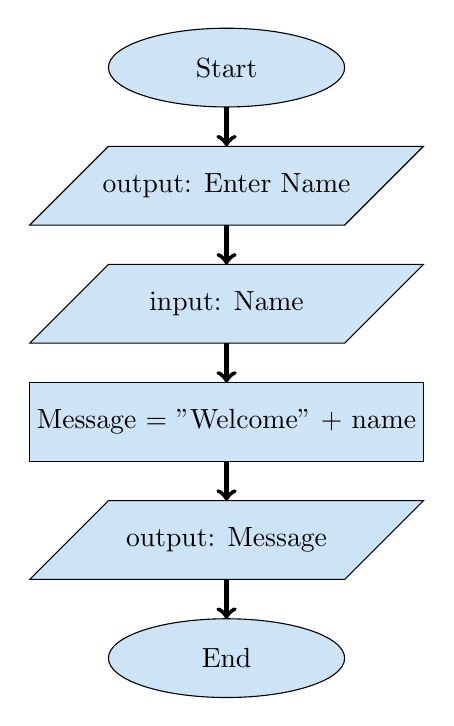
\begin{tikzpicture}
      \draw[fill=theme!20] (5,8) ellipse (1.5cm and .5cm);
      \node at (5,8) {Start};

      \draw[->, ultra thick] (5,7.5) -- (5,7);

      \draw[fill=theme!20] (2.5,6) -- (6.5,6) -- (7.5,7) -- (3.5,7) -- cycle;
      \node at (5,6.5) {output: Enter Name};
      
      \draw[->, ultra thick] (5,6) -- (5,5.5);

      \draw[fill=theme!20] (2.5,4.5) -- (6.5,4.5) -- (7.5,5.5) -- (3.5,5.5) -- cycle;
      \node at (5,5) {input: Name};

      \draw[->, ultra thick] (5,4.5) -- (5,4);

      \draw[fill=theme!20] (2.5,3) rectangle (7.5,4);
      \node at (5,3.5) {Message = "Welcome" + name};

      \draw[->, ultra thick] (5,3) -- (5,2.5);
      
      \draw[fill=theme!20] (2.5,1.5) -- (6.5,1.5) -- (7.5,2.5) -- (3.5,2.5) -- cycle;
      \node at (5,2) {output: Message};

      \draw[->, ultra thick] (5,1.5) -- (5,1);

      \draw[fill=theme!20] (5,.5) ellipse (1.5cm and .5cm);
      \node at (5,.5) {End};

    \end{tikzpicture}
  \end{center}
  \end{example}
\end{minipage} 
  \begin{example}
    \RL{
      قم برسم برناج يدخل فيه المستخدم تاريخ ميلاده
      ثم يتم حساب العمر بناء علي تاريخ الميلاد المدخل
      ثم عرض رسالة تفيد ذلك
     }
    \begin{center}
      ------ \textcolor{Solution}{Solution} ------ 
      \vspace*{.5cm}
      \\
      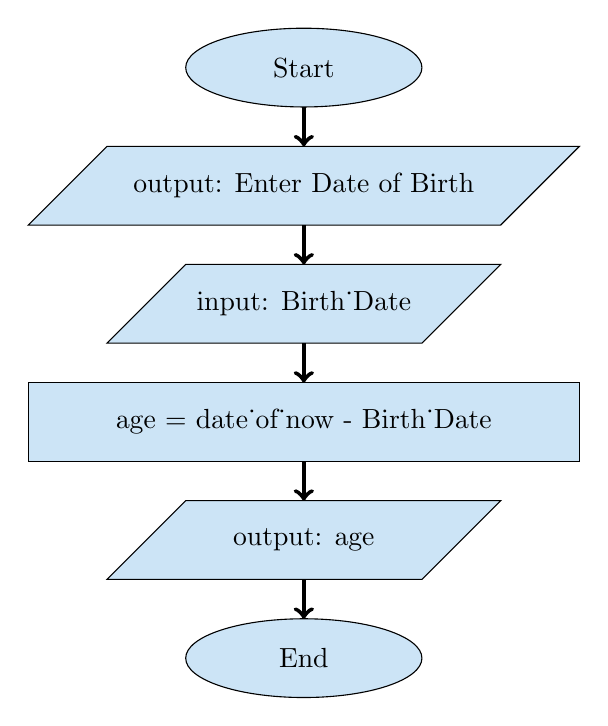
\begin{tikzpicture} 
        \draw[fill=theme!20] (5,8) ellipse (1.5cm and .5cm); 
        \node at (5,8) {Start}; 
   
        \draw[->, ultra thick] (5,7.5) -- (5,7); 
   
        \draw[fill=theme!20] (1.5,6) -- (7.5,6) -- (8.5,7) -- (2.5,7) -- cycle; 
        \node at (5,6.5) {output: Enter Date of Birth}; 
   
        \draw[->, ultra thick] (5,6) -- (5,5.5); 
   
        \draw[fill=theme!20] (2.5,4.5) -- (6.5,4.5) -- (7.5,5.5) -- (3.5,5.5) -- cycle; 
        \node at (5,5) {input: Birth_Date}; 
   
        \draw[->, ultra thick] (5,4.5) -- (5,4); 
   
        \draw[fill=theme!20] (1.5,3) rectangle (8.5,4); 
        \node at (5,3.5) {age  = date_of_now - Birth_Date}; 
   
        \draw[->, ultra thick] (5,3) -- (5,2.5); 
   
        \draw[fill=theme!20] (2.5,1.5) -- (6.5,1.5) -- (7.5,2.5) -- (3.5,2.5) -- cycle; 
        \node at (5,2) {output: age}; 
   
        \draw[->, ultra thick] (5,1.5) -- (5,1); 
   
        \draw[fill=theme!20] (5,.5) ellipse (1.5cm and .5cm); 
        \node at (5,.5) {End}; 
      \end{tikzpicture} 
    \end{center} 
  
\end{example}
\begin{minipage}[h]{1\textwidth}
  \begin{example}
    \RL{قم برسم برنامج يقوم بجمع رقمين ثم يعرض الناتج}
    \begin{center}
      \vspace*{.1cm}
      ------ \textcolor{Solution}{Solution} ------ 
      \\
      \vspace*{.2cm}
      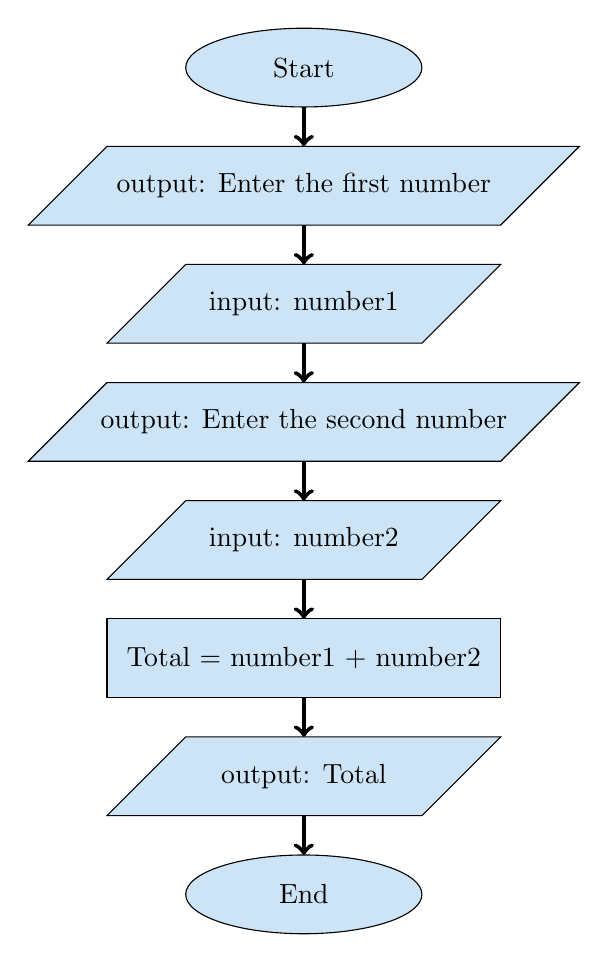
\begin{tikzpicture} 
        \draw[fill=theme!20] (5,8) ellipse (1.5cm and .5cm); 
        \node at (5,8) {Start}; 
   
        \draw[->, ultra thick] (5,7.5) -- (5,7); 
   
        \draw[fill=theme!20] (1.5,6) -- (7.5,6) -- (8.5,7) -- (2.5,7) -- cycle; 
        \node at (5,6.5) {output: Enter the first number}; 
   
        \draw[->, ultra thick] (5,6) -- (5,5.5); 
   
        \draw[fill=theme!20] (2.5,4.5) -- (6.5,4.5) -- (7.5,5.5) -- (3.5,5.5) -- cycle; 
        \node at (5,5) {input: number1}; 
        
        \draw[->, ultra thick] (5,4.5) -- (5,4); 
   
        \draw[fill=theme!20] (1.5,3) -- (7.5,3) -- (8.5,4) -- (2.5,4) -- cycle; 
        \node at (5,3.5) {output: Enter the second number}; 

        \draw[->, ultra thick] (5,3) -- (5,2.5); 
   
        \draw[fill=theme!20] (2.5,1.5) -- (6.5,1.5) -- (7.5,2.5) -- (3.5,2.5) -- cycle; 
        \node at (5,2) {input: number2}; 

        \draw[->, ultra thick] (5,1.5) -- (5,1); 
 
        \draw[fill=theme!20] (2.5,0) rectangle (7.5,1); 
        \node at (5,.5) {Total  = number1 + number2}; 

        \draw[->, ultra thick] (5,0) -- (5,-.5); 
   
        \draw[fill=theme!20] (2.5,-1.5) -- (6.5,-1.5) -- (7.5,-.5) -- (3.5,-.5) -- cycle; 
        \node at (5,-1) {output: Total}; 

        \draw[->, ultra thick] (5,-1.5) -- (5,-2); 
   
        \draw[fill=theme!20] (5,-2.5) ellipse (1.5cm and .5cm); 
        \node at (5,-2.5) {End}; 
        
      \end{tikzpicture} 
      
    \end{center}      
  \end{example}
\end{minipage} 
  \begin{example}
    \RL{قم برسم برنامج يحسب الزيادة في الراتب و هي \LR{10\%} من قيمة المرتب ثم يعرض المرتب بعد الزيادة}
    \begin{center}
      ------ \textcolor{Solution}{Solution} ------ 
      \vspace*{.2cm}
      \\
    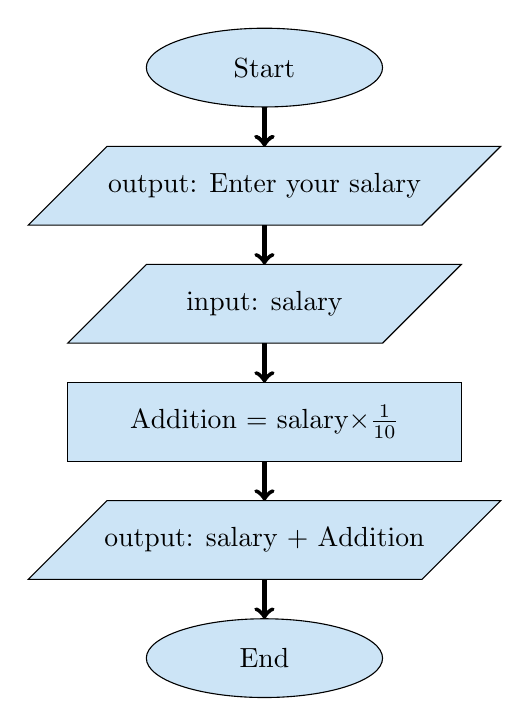
\begin{tikzpicture} 
      \draw[fill=theme!20] (5,8) ellipse (1.5cm and .5cm); 
      \node at (5,8) {Start}; 
 
      \draw[->, ultra thick] (5,7.5) -- (5,7); 

      \draw[fill=theme!20] (2,6) -- (7,6) -- (8,7) -- (3,7) -- cycle; 
      \node at (5,6.5) {output: Enter your salary}; 
 
      \draw[->, ultra thick] (5,6) -- (5,5.5); 
 
      \draw[fill=theme!20] (2.5,4.5) -- (6.5,4.5) -- (7.5,5.5) -- (3.5,5.5) -- cycle; 
      \node at (5,5) {input: salary}; 

      \draw[->, ultra thick] (5,7.5) -- (5,7); 
 
 

      \draw[->, ultra thick] (5,4.5) -- (5,4); 
 
      \draw[fill=theme!20] (2.5,3) rectangle (7.5,4); 
      \node at (5,3.5) {Addition  = salary$\times\frac{1}{10}$}; 
 
      \draw[->, ultra thick] (5,3) -- (5,2.5); 
 
      \draw[fill=theme!20] (2,1.5) -- (7,1.5) -- (8,2.5) -- (3,2.5) -- cycle; 
      \node at (5,2) {output: salary + Addition}; 
 
      \draw[->, ultra thick] (5,1.5) -- (5,1); 
 
      \draw[fill=theme!20] (5,.5) ellipse (1.5cm and .5cm); 
      \node at (5,.5) {End};
    \end{tikzpicture} 
    \end{center} 
  \end{example}
  \begin{minipage}[h]{1\textwidth}
  \begin{example}
    \RL{ارسم برنامج يقوم بحساب محيط و مساحة مربع ثم عرضهم}
    \begin{center}
      \vspace*{.2cm}
      ------ \textcolor{Solution}{Solution} ------ 
      \\
      \vspace*{.3cm}
    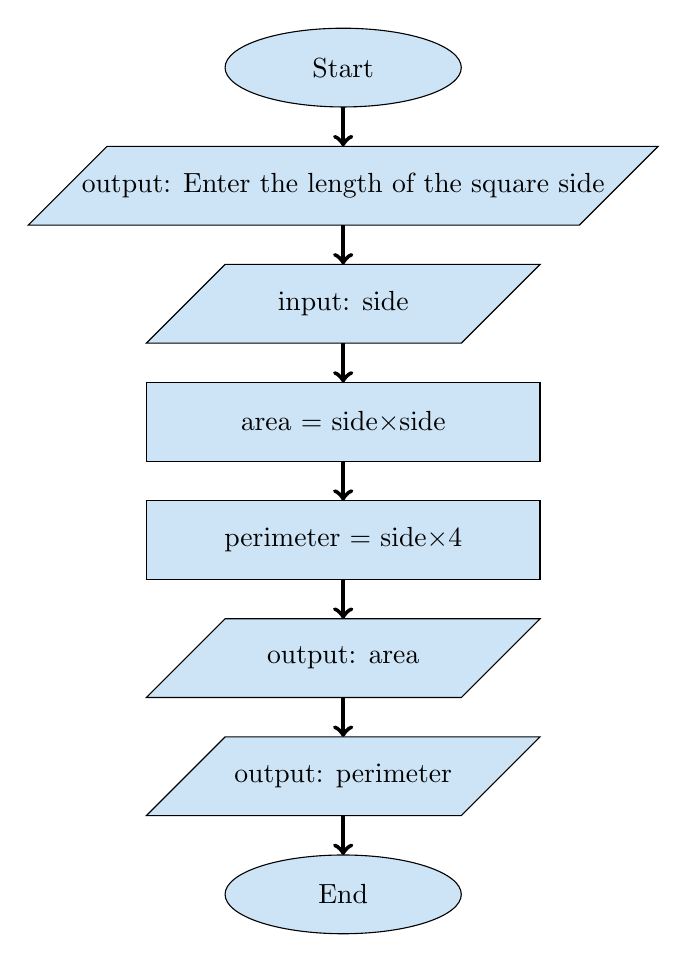
\begin{tikzpicture} 
      \draw[fill=theme!20] (5,8) ellipse (1.5cm and .5cm); 
      \node at (5,8) {Start}; 
 
      \draw[->, ultra thick] (5,7.5) -- (5,7); 
 
 
      \draw[fill=theme!20] (1,6) -- (8,6) -- (9,7) -- (2,7) -- cycle; 
      \node at (5,6.5) {output: Enter the length of the square side}; 
 
      \draw[->, ultra thick] (5,6) -- (5,5.5); 
 
      \draw[fill=theme!20] (2.5,4.5) -- (6.5,4.5) -- (7.5,5.5) -- (3.5,5.5) -- cycle; 
      \node at (5,5) {input: side}; 

      \draw[->, ultra thick] (5,4.5) -- (5,4); 
 
      \draw[fill=theme!20] (2.5,3) rectangle (7.5,4); 
      \node at (5,3.5) {area = side$\times$side}; 

      \draw[->, ultra thick] (5,3) -- (5,2.5); 
 
      \draw[fill=theme!20] (2.5,2.5) rectangle (7.5,1.5); 
      \node at (5,2) {perimeter = side$\times$4}; 

      \draw[->, ultra thick] (5,1.5) -- (5,1); 
 
      \draw[fill=theme!20] (2.5,0) -- (6.5,0) -- (7.5,1) -- (3.5,1) -- cycle; 
      \node at (5,.5) {output: area}; 

      \draw[->, ultra thick] (5,0) -- (5,-.5); 
 
      \draw[fill=theme!20] (2.5,-1.5) -- (6.5,-1.5) -- (7.5,-.5) -- (3.5,-.5) -- cycle; 
      \node at (5,-1) {output: perimeter}; 
      
      \draw[->, ultra thick] (5,-1.5) -- (5,-2); 
 
      \draw[fill=theme!20] (5,-2.5) ellipse (1.5cm and .5cm); 
      \node at (5,-2.5) {End}; 

    \end{tikzpicture}
  \end{center}  
  \end{example}
\end{minipage} 
\newpage
  \begin{example}
    \RL{قم برسم برنامج يدخل فيه المستخدم رقمين و يطبع له الاكبر بينهم}
    \begin{center}
      ------ \textcolor{Solution}{Solution} ------ 

      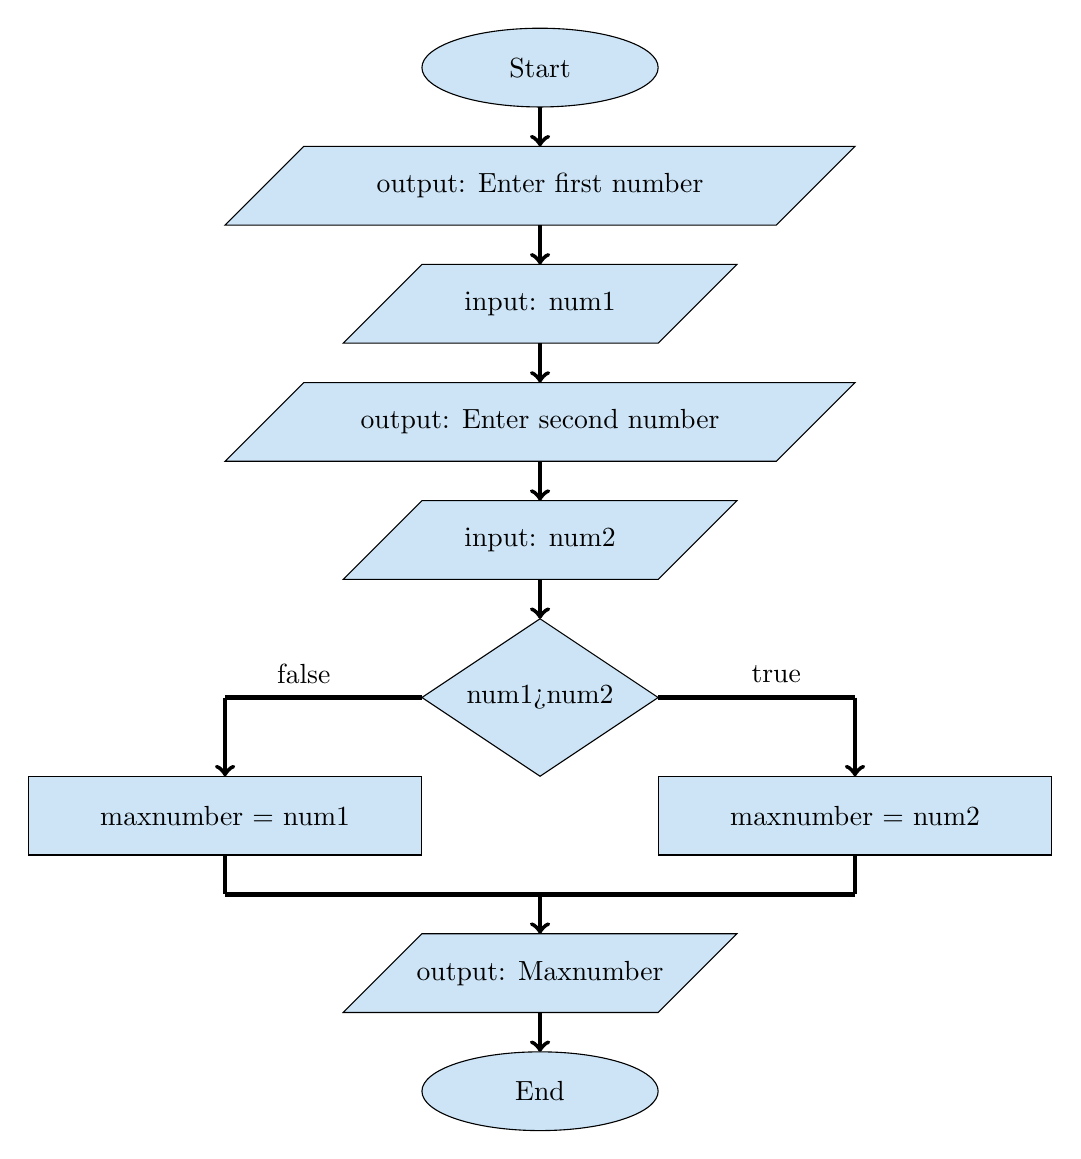
\begin{tikzpicture} 
        \draw[fill=theme!20] (5,8) ellipse (1.5cm and .5cm); 
        \node at (5,8) {Start}; 
   
        \draw[->, ultra thick] (5,7.5) -- (5,7); 
   
   
        \draw[fill=theme!20] (1,6) -- (8,6) -- (9,7) -- (2,7) -- cycle; 
        \node at (5,6.5) {output: Enter first number}; 
   
        \draw[->, ultra thick] (5,6) -- (5,5.5); 
   
        \draw[fill=theme!20] (2.5,4.5) -- (6.5,4.5) -- (7.5,5.5) -- (3.5,5.5) -- cycle; 
        \node at (5,5) {input: num1}; 
  
        \draw[->, ultra thick] (5,4.5) -- (5,4); 
   
        \draw[fill=theme!20] (1,3) -- (8,3) -- (9,4) -- (2,4) -- cycle; 
        \node at (5,3.5) {output: Enter second number}; 
  
        \draw[->, ultra thick] (5,3) -- (5,2.5); 
        
        \draw[fill=theme!20] (2.5,1.5) -- (6.5,1.5) -- (7.5,2.5) -- (3.5,2.5) -- cycle; 
        \node at (5,2) {input: num2}; 
  
        \draw[->, ultra thick] (5,1.5) -- (5,1); 
   
        \draw[fill=theme!20] (3.5,0) -- (5,1) -- (6.5,0) -- (5,-1) -- cycle;
        \node at (5,0) {num1>num2};

        \draw[-, ultra thick] (3.5,0) -- (1,0); 
        \node at (2,0.3) {false};
        \draw[->, ultra thick] (1,0) -- (1,-1); 
        \draw[-, ultra thick] (6.5,0) -- (9,0); 
        \node at (8,0.3) {true};
        \draw[->, ultra thick] (9,0) -- (9,-1); 
        
        \draw[fill=theme!20] (-1.5 ,-1) rectangle (3.5,-2); 
        \node at (1,-1.5) {maxnumber = num1}; 
        
        \draw[fill=theme!20] (6.5 ,-1) rectangle (11.5,-2); 
        \node at (9,-1.5) {maxnumber = num2}; 
        
        \draw[-, ultra thick] (9,-2) -- (9,-2.5); 
        \draw[-, ultra thick] (9,-2.5) -- (1,-2.5); 
        \draw[-, ultra thick] (1,-2) -- (1,-2.5); 
        \draw[->, ultra thick] (5,-2.5) -- (5,-3); 

        \draw[fill=theme!20] (2.5,-4) -- (6.5,-4) -- (7.5,-3) -- (3.5,-3) -- cycle; 
        \node at (5,-3.5) {output: Maxnumber}; 
        
        \draw[->, ultra thick] (5,-4) -- (5,-4.5); 
   
        \draw[fill=theme!20] (5,-5) ellipse (1.5cm and .5cm); 
        \node at (5,-5) {End}; 
      \end{tikzpicture}

    \end{center}  
  \end{example}




  \chapterimage{chapters_cover.jpg}
  \chapter{Introduction to Java}
  \thispagestyle{empty}
  \section{Why Java}
  \begin{AR}
    تعتبر لغة جافا واحدة من اللغات البرمجية الشهيرة والمستخدمة على نطاق واسع في تطوير البرمجيات وتطبيقات الويب والتطبيقات المحمولة. هناك عدة أسباب تجعل تعلم لغة جافا مفيدًا:
    
    \LR{\textcolor{theme}{- 1}} شيوع الاستخدام: جافا تستخدم في مجموعة متنوعة من المجالات بما في ذلك تطوير تطبيقات الويب والهواتف المحمولة والتطبيقات المؤسسية وأنظمة تشغيل الحاسوب والألعاب وغيرها. لذا، إذا كنت ترغب في العمل في أي من هذه المجالات، فإن مهارة جافا قد تكون لها قيمة كبيرة
\\    
    \LR{\textcolor{theme}{- 2}} لغة مستقلة المنصة : جافا معروفة بقدرتها على العمل على مختلف الأنظمة الحاسوبية والمنصات، مما يجعلها لغة مستقلة عن النظام. هذا يعني أنك يمكن أن تكتب تطبيقًا مرة واحدة باستخدام جافا وتشغيله على مجموعة متنوعة من الأجهزة والأنظمة 
\\
    \LR{\textcolor{theme}{- 3}} سهولة القراءة والكتابة: جافا تستخدم بنية بسيطة وصريحة، مما يسهل قراءة وكتابة الكود بها. هذا يسهل عملية التعلم للمبتدئين ويجعل الصيانة أسهل على المدى الطويل
\\
    \LR{\textcolor{theme}{- 4}} أمان وسلامة البرمجة: جافا توفر بيئة تشغيل آمنة وتحتوي على ميزات تحسين أمان البرامج، مما يقلل من احتمالية حدوث ثغرات أمنية وأخطاء برمجية
\\
    \LR{\textcolor{theme}{- 5}} دعم واسع للمجتمع: تمتلك جافا مجتمعًا كبيرًا من المطورين والمستخدمين الذين يقدمون دعمًا وموارد تعليمية وأدوات تطوير متنوعة. هذا يعني أنه يمكنك العثور بسهولة على مساعدة وموارد عند مواجهة تحديات في البرمجة بجافا
\\
    \LR{\textcolor{theme}{- 6}} فرص العمل: نظرًا لشيوع استخدام جافا في مجموعة متنوعة من المجالات التقنية، فإن مهارة البرمجة باستخدام جافا قد تفتح لك فرص عمل واسعة في صناعة تكنولوجيا المعلومات

    بشكل عام، تعلم لغة جافا قد يكون له تأثير إيجابي كبير على مستقبلك المهني في مجال تطوير البرمجيات وتقنية المعلومات
  \end{AR}
  \newpage
  \subsection{Ups and Downs of Java }
  \begin{AR}
    لغة جافا لها العديد من المميزات والعيوب، وهنا سأقدم لك نظرة عامة عنها:
\\
    مميزات لغة جافا:
\\  
\ \ \LR{\textcolor{theme}{- 1}}    منصة مستقلة: تمتاز جافا بقدرتها على العمل على مختلف الأنظمة والمنصات، مما يجعلها مستقلة تمامًا عن النظام. يمكن للتطبيقات الجافا أن تعمل على أي نظام يدعم بيئة تشغيل جافا  
\\ 
\ \ \LR{\textcolor{theme}{- 2}}    أمان البرمجة: تم تصميم جافا بطريقة تسهم في تحسين أمان البرمجة. توفر العديد من الميزات التي تقلل من احتمالية حدوث ثغرات أمنية مثل إدارة الذاكرة
\\ 
\ \ \LR{\textcolor{theme}{- 3}}    مجتمع مطورين ضخم: تتمتع جافا بمجتمع كبير من المطورين والمستخدمين، وهذا يعني وجود مجتمع نشط يقدم دعمًا وموارد تعليمية وأدوات تطوير متنوعة
\\ 
\ \ \LR{\textcolor{theme}{- 4}}    أداء جيد: بفضل تحسينات تقنية \LR{JIT (Just-In-Time)} وأدوات الأداء المتاحة، يمكن لتطبيقات جافا أن تحقق أداءً جيدًا على مستوى النظام
\\ 
\ \ \LR{\textcolor{theme}{- 5}}    معالجة الاستثناءات: تمتلك جافا نظامًا قويًا لمعالجة الاستثناءات يساعد في التعامل مع الأخطاء والمشاكل بطريقة منظمة ومناسبة

    عيوب لغة جافا:
\\
\ \ \LR{\textcolor{theme}{- 1}}    تطبيقات معقدة: في بعض الأحيان، يمكن أن تؤدي هندسة البرمجيات باستخدام جافا إلى إنشاء تطبيقات معقدة \LR{)}بمعنى أنها تستهلك موارد كبيرة\LR{(}، خاصةً إذا لم يتم التصميم بعناية  
\\
\ \ \LR{\textcolor{theme}{- 2}}    تعقيد بعض المفاهيم: تحتوي جافا على بعض المفاهيم المتقدمة مثل التعامل مع المواضيع والتخيير \LR{(Concurrency)} والتعامل مع الذاكرة، وقد يكون هذا معقدًا لبعض المبتدئين
\\
\ \ \LR{\textcolor{theme}{- 3}}    حجم الكود: في بعض الأحيان، قد تحتاج لكتابة كمية كبيرة من الكود في جافا مقارنة ببعض اللغات الأخرى لتحقيق نفس الوظائف
\\
\ \ \LR{\textcolor{theme}{- 4}}    تحديثات اللغة: بسبب وجود إصدارات مختلفة من جافا، قد يكون من الصعب الحفاظ على تحديثات اللغة ومعرفة الميزات الجديدة 
  
    في النهاية لغة جافا تعتبر خيارًا جيدًا للأشخاص الجدد في تعلم البرمجة، وذلك لانها
    سهلة القراءة و الكتابة و يوجد العديد من الموارد التعليمية لها 
    و مجتمعها نشط و يوجد لها العديد من بيئات التطوير المتكاملة 
    \LR{(IDE)} مثل \LR{Eclipse} و\LR{IntelliJ IDEA} و\LR{NetBeans} والتي تساعدك في كتابة واختبار الكود بشكل سهل
    و تحتوي علي جميع مفاهيم البرمجة الاساسية و من ضمنها و اهمها \LR{OOP (object oriented programming)} او البرمجة الشيئية و التي سوف يتم مناقشتها لاحقا
  \end{AR}
\begin{figure*}[b]
  \begin{enrichment*}{IDE \RL{بيئة تطوير متكاملة}}
    \begin{AR}
      \LR{IDE} هو اختصار لعبارة \LR{"Integrated Development Environment"} او بيئة تطوير متكاملة هي عبارة عن برمجيات تُستخدم من قبل المطورين لتطوير وإدارة تطبيقات البرمجة. توفر ال\LR{IDE} بيئة متكاملة للكتابة وتحرير الاكواد، وتصحيح الأخطاء، واختبار وتصحيح البرامج، وإدارة الإصدارات، وبناء وتجميع التطبيقات، والتفاعل مع قواعد البيانات.
    \end{AR}
  \end{enrichment*}
\end{figure*}
  \newpage
  \section{Getting Started}
  \begin{AR}
    قبل البدء في لغة الجافا هناك ثلاث مفاهيم علينا معرفتهم
  \end{AR}

  \begin{definition}{JRE (Java Runtime Environment)}
    \begin{AR}
     \LR{JRE} هو اختصار لـ \LR{Java Runtime Environment}، وهو بيئة تشغيل لتطبيقات جافا. يتضمن \LR{JRE} مكتبات البرامج والملفات الضرورية التي يحتاجها نظام التشغيل لتشغيل تطبيقات جافا المختلفة. عندما تقوم بتشغيل تطبيق جافا، فإن \LR{JRE} تكون المسؤولة عن تحميل وتنفيذ التطبيق
    \end{AR}
  \end{definition}

  \begin{definition}{JVM (Java Virtual Machine)}
    \begin{AR}
      \LR{JVM} هو اختصار لـ \LR{Java Virtual Machine}، وهي آلة افتراضية تقوم بتنفيذ تعليمات البرمجة الخاصة بلغة جافا. تقوم \LR{JVM} بتحميل الاوامر المكتوبة بلغة جافا وتنفيذها على النظام الفعلي \LR{)}مثل نظام التشغيل\LR{(}. تعتبر \LR{JVM} مفتاحية في جعل تطبيقات جافا قابلة للتشغيل عبر منصات مختلفة، حيث توفر وسيطًا بين الاكواد ونظام التشغيل
    \end{AR}
  \end{definition}

  \begin{definition}{JDK (Java Development Kit)}
    \begin{AR}
      \LR{JDK} هو اختصار لـ \LR{Java Development Kit}، وهي مجموعة من الأدوات والمكتبات التي تسمح للمطورين بتطوير واختبار وتشغيل تطبيقات جافا. يتضمن \LR{JDK} ملفات \LR{JRE} والأدوات المطلوبة للتطوير مثل مترجم الجافا \LR{(javac)} وأداة التشغيل \LR{(java)} ومكتبات التطوير. ببساطة، \LR{JDK} هو مجموعة شاملة لتطوير تطبيقات جافا
    \end{AR}
  \end{definition}
  \begin{AR}
    عند تنزيل ال \LR{JDK} فأنه يتم تنزيل معاها كلا من \LR{JVM} و \LR{JRE} 
  \end{AR}
  \subsection{Our First Project}
  \begin{AR}
    بعد تحميل و تسطيب ال \LR{JDK} و ال\LR{IDE} الذي سوف نقوم بالعمل عليه سواء كان \LR{Netbeans} او \LR{Eclipse} او \LR{IntelliJ IDEA} لن يشكل اي فارق استخدام اي واحد

    المستخدم في الشرح هو \LR{JDK 20} احدث نسخة موجودة في تاريخ 31 اغسطس 2023 و \LR{Apache Netbeans}

    لعمل مشروع جديد في \LR{NetBeans} قم بالضغط علي علامة \LR{new project} اعلي يسار الشاشة
  \end{AR}
  \begin{center}
    
\includegraphics[scale=.7]{newProjecticon.png}  
  \end{center}
  \begin{AR}
    ثم اختيار \LR{Java application} بعد اختيار \LR{Java with ant}
  \end{AR}
  \begin{center}
    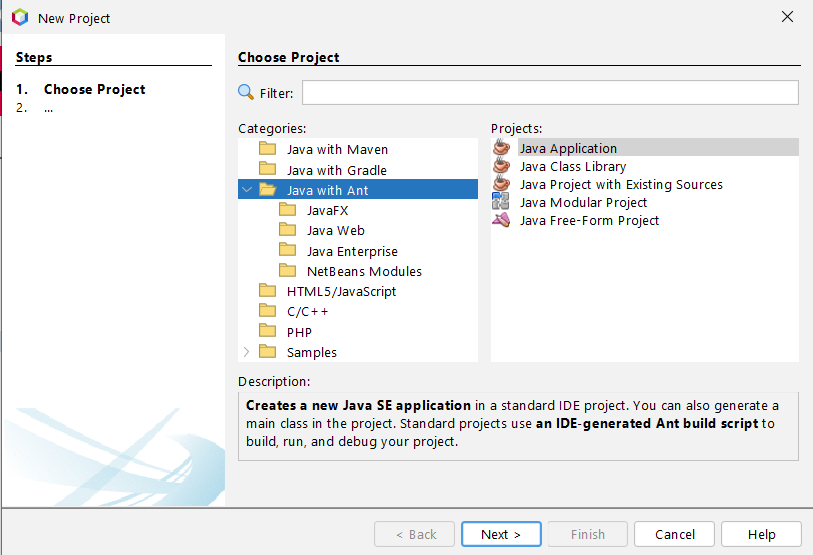
\includegraphics[scale=.5]{Java_app.png}  
  \end{center}
  \newpage
  \begin{AR}
    ثم اختيار اسم المشروع 
  \end{AR}
  \begin{center}
    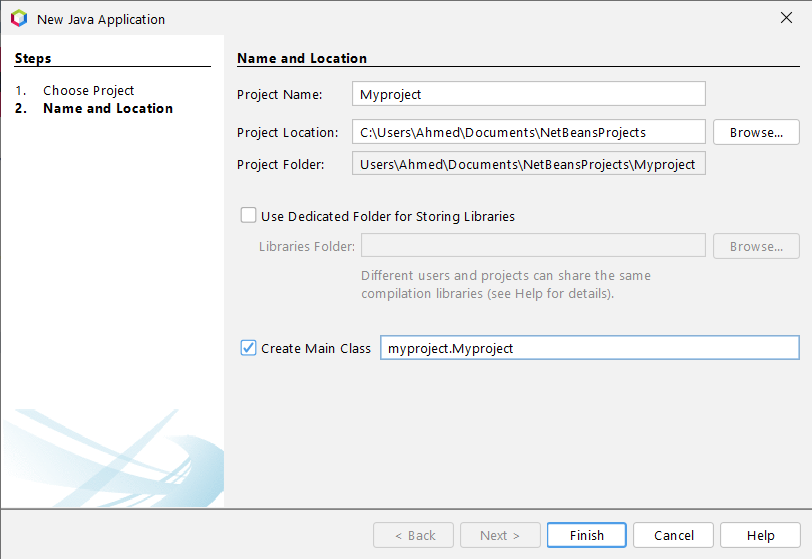
\includegraphics[scale=.4]{naming the project.png}  
  \end{center}
  
  \begin{AR}
    سوف تجد انه قام بعمل \LR{Package} بنفس اسم المشروع و قام ايضا بعمل \LR{Class} بنفس الاسم و قام بكتابة ال \LR{main method} الذي سوف يتم تنفيذ الاكواد بداخلها
    لا تجعل بعض الالفاظ تحيرك او تربكك سوف يتم شرح كل شئ في وقته المناسب 
  \end{AR}
  \begin{center}
    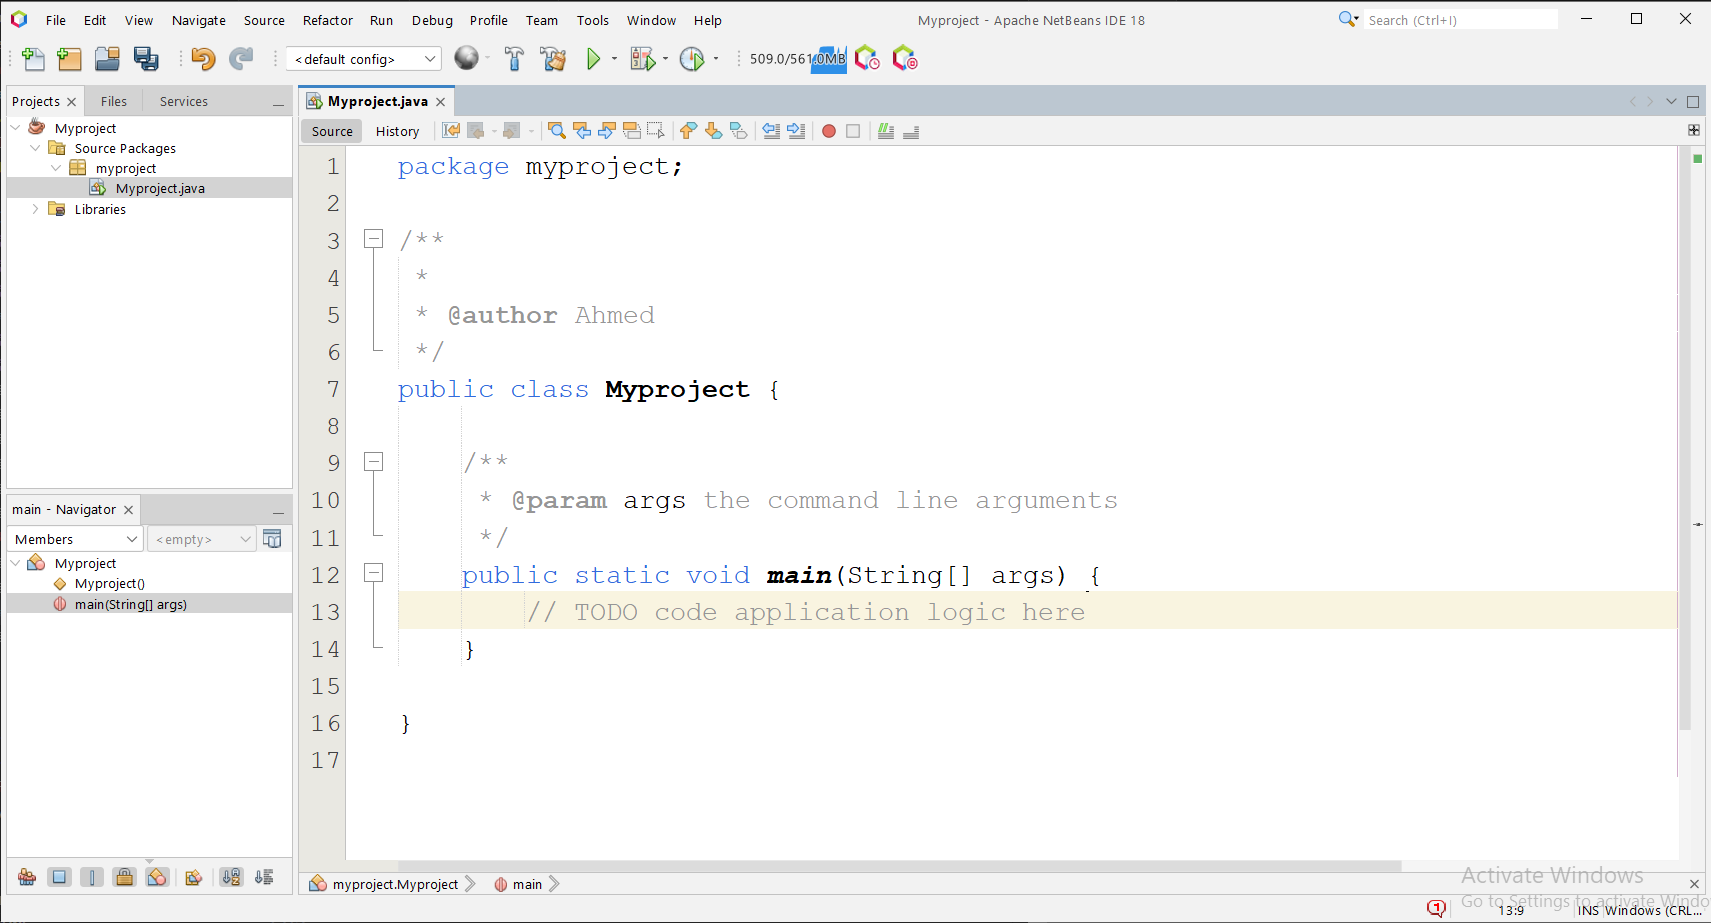
\includegraphics[scale=.35]{homepage.png}  
  \end{center}
  
  \begin{AR}
    ما يهمنا في البداية هو الجزء المكتوب فيه \LR{// TODO code application logic here} حيث ان هذا هو مكان كتابة الاكواد التي سوف تنفذ

    مثلا اذا اردت طباعة شئ ما اقوم بكتابة 
  \end{AR}
  \begin{minted}{java}
    System.out.println("Hello world!")
  \end{minted}
  \begin{AR}
    في ذلك المكان ثم اضغط علي زر ال\LR{Run} او اضغط علي زر ال\LR{F6} في الكيبورد 
  \end{AR}
  \begin{center}
    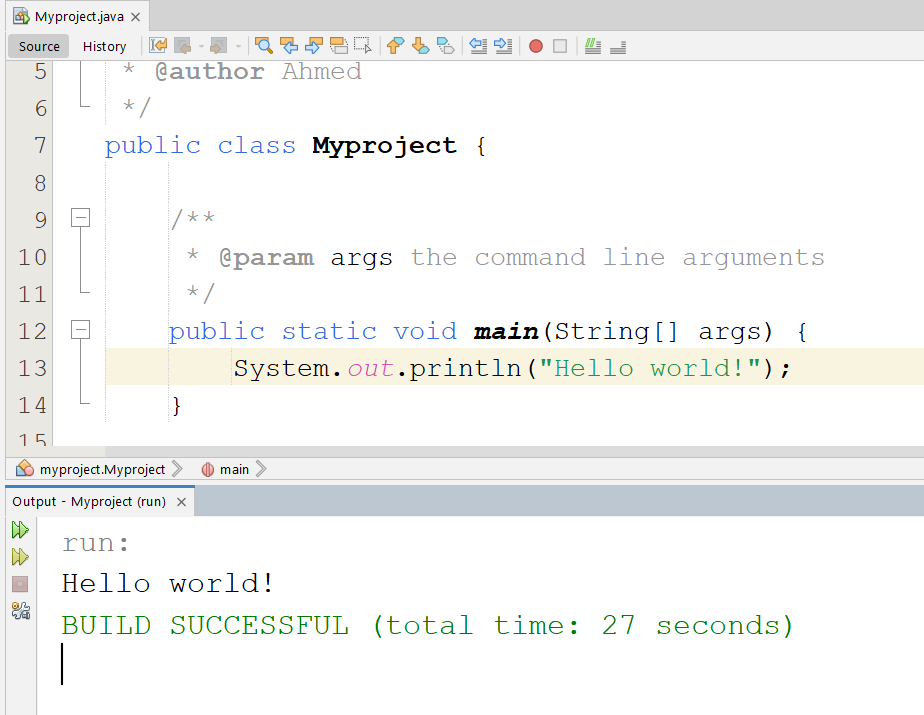
\includegraphics[scale=.5]{output1.png}  
  \end{center}
  \begin{AR}
    كما في الصورة تم طباعة جملة \LR{Hello world!} كما هو مطلوب
  \end{AR}
\newpage
  \section{Data Type}
  \begin{AR}
    الان سوف نترك كتابة الاكواد لبعض الوقت و نتحدث عن البيانات و انواعها
  \end{AR}
  

  \begin{center}
  %\rowcolors{2}{theme!80}{theme!30}
  \begin{tabular}{ |c c c c| } 
    \hline
    Data Type & \RL{الحجم}  &  \RL{الوصف} &  \RL{القيم الافتراضية} \\
    \hline
    \textcolor{red}{byte} & 1 byte & 127 \RL{الي} -128 \RL{تستخدم لتخزين ارقام صحيحة بين}  & 0 \\
    \hline
    \textcolor{red}{short} & 2 byte & 32,767 \RL{الي} -32,768 \RL{تستخدم لتخزين ارقام صحيحة بين} & 0  \\
    \hline
    \textcolor{red}{int} & 4 byte & $2^{31}-1$ \RL{الي} $-2^{31}$ \RL{تستخدم لتخزين ارقام صحيحة بين} & 0 \\
    \hline
    \textcolor{red}{long} & 8 byte & $2^{63}-1$ \RL{الي} $-2^{63}$ \RL{تستخدم لتخزين ارقام صحيحة بين} & 0L \\
    \hline
    \textcolor{red}{float} & 4 byte & \RL{يخزن الأعداد الكسرية كافية لتخزين 6 إلى 7 أرقام عشرية} & 0.0f \\
    \hline
    \textcolor{red}{double} & 8 byte & \RL{يخزن الأعداد الكسرية يكفي لتخزين 15 رقمًا عشريًا} & 0.0d \\
    \hline
    \textcolor{red}{boolean} & 1 byte & false \RL{او} True \RL{يخزن القيم المنطقية }  & false \\
    \hline
    \textcolor{red}{char} & 2 byte & ASCII \RL{يخزن الحروف و قيم}  & '0' or '$\backslash$u0000' \\
    \hline
    \textcolor{red}{String} & \RL{متغير} & \RL{يستخدم لتخزين النصوص}  & null \\
    \hline
  \end{tabular}
\end{center}

\begin{AR}
  هناك انواع اخري سوف يتم مناقشتها في المستقبل لكن سوف نكتفي حاليا بهذا القدر حيث ان هذه الانواع هي الاساسية 

  قد يخطر علي بال البعض لماذا يوجد \LR{6} انواع مختلفة فقط للارقام لماذا لا نستخدم نوع \LR{double} لاي معلومة رقمية نريد تخزينها 
\\
  الان لننظر لمثال من الحياة الحقيقة اذا اردت تخزين عمر شخص ما بالنظر لانواع البيانات السابقة بنظرك ايهم افضل لتخزينه
  \\
  سوف تجد انه اذا تم تخزين هذه القيمة في متغير نوعه \LR{double} سوف يحجز مساحة كبيرة في الذاكرة بدون داعي
  بينما يمكن تخزينه في متغير من نوع \LR{byte} سوف يكون اكثر عملية
  
  علي مدار الشرح لن نضع في الاعتبار هذا الامر عندما نريد تخزين رقم صحيح سوف نستخدم \LR{int} و للارقام النسبية \LR{double} بدون الوضع في الاعتبار المساحة 
  لان هذا مجرد تعليم لكن عند العمل علي المشاريع الحقيقة لابد من الوضع في الاعتبار هذا الامر و دراسته جيدا قبل اختيار انواع المتغيرات
\end{AR}



  \subsection{Variables}
  \begin{AR}
    المتغيرات \LR{(Variables)} هي عبارة عن رموز تُستخدم في البرمجة لتخزين البيانات والمعلومات في الذاكرة خلال تنفيذ البرنامج. تُعتبر المتغيرات وسيلة لتخزين القيم والمعلومات التي يمكن أن يتم التلاعب بها واستخدامها أثناء تنفيذ البرنامج

    عندما تقوم بتعريف متغير في لغة برمجة، فإنك تقوم بتخصيص مساحة في الذاكرة لتخزين قيمة محددة. يمكن أن تكون هذه القيمة عددًا، نصًا، قيمة منطقية \LR{false)} أو \LR{(true}، أو أي نوع آخر من البيانات حسب نوع المتغير

    على سبيل المثال، إذا كنت تريد تخزين عمر شخص ما في برنامجك، يمكنك تعريف متغير يسمى \LR{"age"} وتخصيص مساحة في الذاكرة لتخزين قيمة العمر فيه. وبعد ذلك، يمكنك استخدام هذا المتغير للقيام بالعمليات والحسابات على العمر

    قبل استخدام المتغيرات في البرمجة، عادة ما يجب تحديد نوع المتغير وإعطائه اسمًا فريدًا. عندما ترغب في تخزين قيمة جديدة في المتغير، يمكنك تعيينها له باستخدام عملية تعيين. في لغة برمجة \LR{Java}، يمكنك كتابة:
  \end{AR}

  \begin{minted}{java}
    String name = "Ahmed"; 
    int Age = 30;
  \end{minted}

  \begin{AR}
    هناك قواعد في لغة ال \LR{Java} يجب اتباعها عند تعريف متغير حتي لا يحدث خطأ

\\
\ \ \LR{\textcolor{theme}{- 1}}    أسماء المتغيرات \LR{(Identifiers)}: 
يجب أن تبدأ أسماء المتغيرات بحرف \LR{a-z)} أو \LR{(A-Z} أو الشرطة السفلية \LR{(_)} أو الدولار \LR{(\$)} يمكن أن تحتوي بقية الأحرف في الاسم على أحرف \LR{a-z)} أو \LR{(A-Z}، أرقام \LR{(0-9)}، الشرطة السفلية \LR{(_)}، والدولار \LR{(\$)}.
لكن غير مقبول بداية اسم متغير برقم او استخدام اي رمز اخر 
\\
\ \ \LR{\textcolor{theme}{- 2}}   حالة الأحرف \LR{(Case Sensitivity)}:
جافا حساسة لحالة الأحرف، مما يعني أن \LR{"myVariable"} و \LR{"myvariable"} و \LR{"MyVariable"} يعتبرون مختلفين  
\\
\ \ \LR{\textcolor{theme}{- 3}}    الكلمات المحجوزة \LR{(Reserved Keywords)}:
لا يمكن استخدام الكلمات المحجوزة في جافا كأسماء للمتغيرات. مثل: \LR{"int"} , \LR{"if"} , \LR{"while"} , إلخ
و الكلمات المحجوزة هي الكلمات التي لها معني او استخدام في اللغة 
\\
\ \ \LR{\textcolor{theme}{- 4}}    أنواع المتغيرات \LR{(Data Types)}
يجب تحديد نوع المتغير عند تعريفه. مثل: \LR{"int"} , \LR{"double"} , \LR{"String"}  وما إلى ذلك
\\
\ \ \LR{\textcolor{theme}{- 5}} اسم المتغير يجب ان يكون متصل اي ان المسافات ممنوعة
  \end{AR}
  \subsection{Assignment Operators}
  \begin{AR}
    في لغة الجافا، تُستخدم \LR{Assignment Operators} لتعيين قيمة لمتغير. هذه العوامل تُعد من العناصر الأساسية في البرمجة وتُسهم في تحديد القيم المخزنة في المتغيرات. إليك قائمة ببعض عوامل التخصيص في لغة الجافا وشرح عن كيفية استخدامها
    \\
    \ \ \LR{\textcolor{theme}{- 1}}   \LR{(=)} : يُستخدم لتعيين قيمة إلى متغير. على سبيل المثال
  \end{AR}
  \begin{minted}{java}
      int x = 10; 
  \end{minted}
  \begin{AR} 
  في هذا المثال اقوم بجعل قيمة  \LR{x} تساوي \LR{10} اي انه عند منادة المتغير \LR{x} ثانية في اي جزء من الكود عند تنفيذ الكود سوف يتم تبديلها ب \LR{10}
    \\
    \ \ \LR{\textcolor{theme}{- 2}}  \LR{(+=)}  : يستخدم لاضافة قيمة الي قيمة المتغير الاصلي و جعل الناتج هو قيمة المتغير الحالي مثال:
  \end{AR}
  \begin{minted}{java}
    int y = 5;
    y += 3;
  \end{minted}
  \begin{AR}
    في هذا المثال قيمة \LR{y} الاصلية هي \LR{5} و بعد تنفيذ الكود \LR{y += 3} سوف تتجد قيمتها اصبحت \LR{5+3=8} و هذه هي قيمة \LR{y} الحالية
    و هذا الكود يعادل كتابة \LR{y = y + 3}
    \\
    \ \ \LR{\textcolor{theme}{- 3}}    \LR{(-=)} : مثل المعامل السابق لكن هذه المرة ينقص من قيمة المتغير
  \end{AR}
  \begin{minted}{java}
    int y = 5;
    y -= 3;
  \end{minted}
  \begin{AR}
    في هذا المثال قيمة \LR{y} الاصلية هي \LR{5} و بعد تنفيذ الكود \LR{y -= 3} سوف تصبح \LR{5-3=2} و هذه هي قيمة \LR{y} الحالية
    و هذا الكود يعادل كتابة \LR{y = y - 3}
    \\
    \ \ \LR{\textcolor{theme}{- 4}}    \LR{(*=)} : مثل المعامل السابق لكن هذه المرة يضاعف من قيمة المتغير
  \end{AR}
  \begin{minted}{java}
    int y = 5;
    y *= 3;
  \end{minted}
  \begin{AR}
    في هذا المثال قيمة \LR{y} الاصلية هي \LR{5} و بعد تنفيذ الكود \LR{y *= 3} سوف تصبح \LR{5*3=15} و هذه هي قيمة \LR{y} الحالية
    و هذا الكود يعادل كتابة \LR{y = y * 3}
    \\
    \ \ \LR{\textcolor{theme}{- 5}} \LR{(/=)} : مثل المعامل السابق لكن هذه المرة يقسم المتغير علي قيمة ما
  \end{AR}
  \begin{minted}{java}
    int y = 10;
    y /= 2;
  \end{minted}
  \begin{AR}
    في هذا المثال قيمة \LR{y} الاصلية هي \LR{10} و بعد تنفيذ الكود \LR{y /= 3} سوف تتجد قيمتها لتصبح \LR{10/2=5} و هذه اصبحت هي قيمة \LR{y} الحالية
    و هذا الكود يعادل كتابة \LR{y = y / 3}
    \\
    \ \ \LR{\textcolor{theme}{- 6}} \LR{(\%=)} : هذا المعامل يستخدم للحصول علي باقي قسمة المتغير علي قيمة اخري
  \end{AR}
  \begin{minted}{java}
    int y = 5;
    y %= 3;
  \end{minted}
  \begin{AR}
    في هذا المثال قيمة \LR{y} الاصلية هي \LR{5} و بعد تنفيذ الكود \LR{y \%= 3} سوف تصبح \LR{5\%3=2} و هذه هي قيمة \LR{y} الحالية
    و هذا الكود يعادل كتابة \LR{y = y \% 3}


    هذه هي أمثلة بسيطة على كيفية استخدام عوامل التخصيص في لغة الجافا. يمكنك استخدام هذه العوامل لتعديل قيم المتغيرات وإجراء العمليات البسيطة عليها بطرق مختلفة.

    هناك بعض الملاحظات علي عوامل التخصيص هذه عليك اخذها في الاعتبار 

\\
\ \ \LR{\textcolor{theme}{- 1}}    \LR{(-=)} و \LR{(*=)} و \LR{(/=)} \LR{(\%=)} يستخدموا فقط مع الارقام لا يمكنك استخدامها مع اي نوع اخر من المتغيرات 
\\
\ \ \LR{\textcolor{theme}{- 2}}    \LR{(+=)} يمكن استخدام هذا المعامل مع النصوص كالاتي 
\end{AR}
\begin{minted}{java}
  String A = "Hello";
  A += " ";
  A += "world";
  System.out.println(A);
\end{minted}
\begin{AR}
  في ذلك المثال قيمة \LR{A} في البداية \LR{(Hello)} ثم بعد السطر الثاني تصبح \LR{(Hello )} ثم بعد السطر الثالث تصبح \LR{(Hello world)} و عند تنفيذ السطر الرابع يكون هذا هو الناتج 
\end{AR}
\begin{minted}{java}
  Output : Hello world
\end{minted}
\begin{AR}  
\\
\ \ \LR{\textcolor{theme}{- 3}}    عند استخدام \LR{(=)} ف انه يتم تغيير قيمة المتغير الحالية للقيمة الجديدة لكن عند استخدام \LR{(+=)} يتم الاضافة علي القيمة الاصلية للمتغير بدون حذفها 
\end{AR}
\begin{minted}{java}
  String A = "Ahmed ";
  A += "mohamed";
  System.out.println(A);
  A = "Ali";
  System.out.println(A);
\end{minted}
\begin{AR}  
  بعد تنفيذ الكود السابق سوف يتم طباعة الاتي
\end{AR}
\begin{minted}{java}
  Output : Ahmed mohamed
           Ali
\end{minted}
\begin{AR} 
  ما حدث هو انه في البداية قيمة \LR{A} تساوي \LR{(Ahmed)} بعدها اقوم باضافة \LR{(mohamed)} لتصبح \LR{(Ahemd mohamed)} و اقوم بطباعتها ثم بعد ذلك اقوم بتعيين قيمة جديدة لل \LR{A} و اجعله يساوي \LR{(Ali)} ثم اقوم بطباعته
  \\
\ \ \LR{\textcolor{theme}{- 4}} لا يمكنك تعيين قيمة لمتغير بغير نوعه بمعني اذا قمت بتعريف متغير نوعه \LR{int} ف اذا قمت بجعل هذا المتغير يساوي نص او قيمة منطقية او قيمة كسرية سوف فأن البرنامج سوف يقوم بطباعة \LR{Error} او \LR{Exception}
\end{AR}
\newpage
\subsection{Arithmetic Operators}
\begin{AR}
في لغة البرمجة جافا، تُستخدم العوامل الحسابية \LR{(Arithmetic Operators)} لأداء العمليات الرياضية الأساسية على الأرقام. تتضمن هذه العوامل الحسابية عدة عمليات مثل الجمع والطرح والضرب والقسمة وغيرها. فيما يلي قائمة بأهم العوامل الحسابية في جافا:
\\
\ \ \LR{\textcolor{theme}{- 1}} جمع \LR{(+)}: يُستخدم لجمع عددين معاً و تستخدم ايضا لدمج النصوص ببعضها
\\
\ \ \LR{\textcolor{theme}{- 2}} طرح \LR{(-)}: يُستخدم لطرح عدد من عدد أخرى
\\
\ \ \LR{\textcolor{theme}{- 3}} ضرب \LR{(*)}: يُستخدم لضرب عددين معاً
\\
\ \ \LR{\textcolor{theme}{- 4}}قسمة \LR{(/)}: يُستخدم لقسمة عدد على عدد أخرى
\\
\ \ \LR{\textcolor{theme}{- 5}} باقي القسمة \LR{(\%)}: يُستخدم للحصول على باقي القسمة بين عددين
\end{AR}

\subsection{logical operators}
\begin{AR}
  في لغة البرمجة جافا، تُستخدم العوامل المنطقية \LR{(Logical Operators)} للتحقق من الشروط المنطقية وإجراء العمليات المنطقية على القيم المنطقية \LR{false)} أو \LR{(true}. تساعد هذه العوامل في إجراء قرارات برمجية مبنية على توافق الشروط المنطقية. فيما يلي قائمة بالعوامل المنطقية الرئيسية في جافا:
  \\
\ \ \LR{\textcolor{theme}{- 1}}\LR{(\&\&) AND} و : يُستخدم للتحقق من صحة شرطين على السواء. إذا كان كلا الشرطين صحيحين، فإن النتيجة ستكون صحيحة
\\
\ \ \LR{\textcolor{theme}{- 2}}\LR{(||) OR} او : يُستخدم للتحقق من صحة أحد الشروط على الأقل. إذا كان أحد الشروط على الأقل صحيحًا، فإن النتيجة ستكون صحيحة
\\
\ \ \LR{\textcolor{theme}{- 3}}\LR{(!) NOT} عكس : يُستخدم لعكس قيمة الشرط، أي أنه يحول صح إلى خطأ والعكس صحيح
\end{AR}

\begin{table}[h]
  \begin{tabular}{|c|c|c|}
      \hline
      \multicolumn{3}{|c|}{AND}\\ \hline
      \multicolumn{3}{|c|}{X \&\& Y = Z}\\ \hline
      X&Y&Z \\ \hline
      \textcolor{green}{True}&\textcolor{green}{True}&\textcolor{green}{True} \\ \hline
      \textcolor{green}{True}&\textcolor{red}{False}&\textcolor{red}{False} \\ \hline
      \textcolor{red}{False}&\textcolor{green}{True}&\textcolor{red}{False} \\ \hline
      \textcolor{red}{False}&\textcolor{green}{True}&\textcolor{red}{False} \\ \hline
  \end{tabular}
  \hfill
  \begin{tabular}{|c|c|c|}
    \hline
    \multicolumn{3}{|c|}{OR}\\ \hline
    \multicolumn{3}{|c|}{X || Y = Z}\\ \hline
    X&Y&Z \\ \hline
    \textcolor{green}{True}&\textcolor{green}{True}&\textcolor{green}{True} \\ \hline
    \textcolor{green}{True}&\textcolor{red}{False}&\textcolor{green}{True} \\ \hline
    \textcolor{red}{False}&\textcolor{green}{True}&\textcolor{green}{True} \\ \hline
    \textcolor{red}{False}&\textcolor{green}{True}&\textcolor{red}{False} \\ \hline
\end{tabular}
  \hfill
  \begin{tabular}{|c|c|}
    \hline
    \multicolumn{2}{|c|}{NOT}\\ \hline
    \multicolumn{2}{|c|}{!X = Y}\\ \hline
    X&Y \\ \hline
    \textcolor{green}{True}&\textcolor{red}{False} \\ \hline
    \textcolor{red}{False}&\textcolor{green}{True} \\ \hline
\end{tabular}
\end{table}

\begin{AR}
تُستخدم هذه العوامل المنطقية بشكل شائع لبناء تعبيرات منطقية معقدة واتخاذ قرارات برمجية استنادًا إلى تحقق شروط مختلفة. على سبيل المثال، يمكن استخدامها للتحقق من وجود شروط متعددة في الوقت نفسه أو لتفادي تنفيذ الأكواد في حالة عدم تحقق شرط معين
\end{AR}
\par

\subsection{comparison operators}
\begin{AR}
  في لغة البرمجة جافا، تُستخدم عوامل المقارنة 
  \LR{(Comparison Operators)} لمقارنة بين قيم مختلفة والحصول على قيمة منطقية \LR{)}صح أو خطأ\LR{(} تشير إلى نتيجة المقارنة. تُستخدم هذه العوامل للتحقق من العلاقة بين القيم واتخاذ قرارات استنادًا إلى هذه العلاقة. فيما يلي قائمة بالعوامل المقارنة الرئيسية في جافا:
\newpage
  \\
\ \ \LR{\textcolor{theme}{- 1}}  يساوي \LR{(==)}: يُستخدم للتحقق من مساواة قيمتين. إذا كانت القيمتين متساويتين، فإن النتيجة ستكون صحيحة، وإلا ستكون خطأ  
\\
\ \ \LR{\textcolor{theme}{- 2}}    لا يساوي \LR{(!=)}: يُستخدم للتحقق من عدم المساواة بين قيمتين. إذا كانت القيمتين غير متساويتين، فإن النتيجة ستكون صحيحة، وإلا ستكون خطأ
\\
\ \ \LR{\textcolor{theme}{- 3}}    أكبر من \LR{(<)}: يُستخدم للتحقق من أن قيمة أولى أكبر من قيمة ثانية
\\
\ \ \LR{\textcolor{theme}{- 4}}    أصغر من \LR{(>)}: يُستخدم للتحقق من أن قيمة أولى أصغر من قيمة ثانية
\\
\ \ \LR{\textcolor{theme}{- 5}}      أكبر من أو يساوي \LR{(<=)}: يُستخدم للتحقق من أن قيمة أولى أكبر من أو تساوي قيمة ثانية
\\
\ \ \LR{\textcolor{theme}{- 6}}   أصغر من أو يساوي \LR{(>=)}: يُستخدم للتحقق من أن قيمة أولى أصغر من أو تساوي قيمة ثانية
\end{AR}

\subsection{Increment and Decrement operators}

\begin{AR}
  ال \LR{(++)} و ال \LR{(-{}-)} هي عوامل احادية \LR{(unary operators)} تقوم بالتاثير علي متغير واحد فقط و مهمتها زيادة قيمته بمقدار \LR{1} او انقاصها بنفس المقدار

  و تكتب هكذا و تسمي \LR{Postfix}
\end{AR}
\begin{minted}{java}
  int x = 5 ;
  x++;  
\end{minted}
\begin{AR}
  او هكذا و تسمي \LR{Prefix}
\end{AR}
\begin{minted}{java}
  int x = 5 ;
  --x;  
\end{minted}
\begin{AR}
  الفرق بين ال \LR{Postfix} و ال \LR{Prefix} هو فرق في ترتيب عملية الزيادة او النقصان
  مثلا في الكود الاتي 
\end{AR}
\begin{minted}{java}
  int x = 5 ;
  System.out.println(x++);
  System.out.println(x);

  output: 5
          6
\end{minted}
\begin{AR}
  قام الاول بطباعة قيمة ال \LR{x} قبل التغيير ثم غيرها و ظهر هذا التغيير في الطباعة الثانية اما اذا كتبناها بطريقة ال 
  \LR{prefix}
  سنري الاتي 
\end{AR}
\begin{minted}{java}
  int x = 5 ;
  System.out.println(++x);

  output: 6
\end{minted}
\begin{AR}
  كما نري قام الاول بتغيير قيمة ال \LR{x} ثم قام بتنفيذ الطباعة و نفس الشئ ينطبق علي النقصان 
\end{AR}
\begin{minted}{java}
  int x = 5 ;
  System.out.println(x--);
  System.out.println(x);

  output: 5
          4
--------------------------------------
  int x = 5 ;
  System.out.println(--x);

  output: 4
\end{minted}

\subsection{Input and Scanner}
\begin{AR}
  الي هذه اللحظة كل ما تعلمناه هو تعريف بعض المتغيرات و بعض العمليات عليهم و كيف اظهر رسالة للمستخدم لكن ماذا لو اردنا استقبال شئ من المستخدم 
  نريد ان نجعل برنامجنا \LR{Dynamic} اي متفاعل مع المتسخدم و ليس \LR{Static}
  لجعل البرنامج الخاص بنا يستقبل قيمة من المستخدم نحن نستخدم متغير من نوع خاص يسمي \LR{Scanner} و له طريقة تعريف خاصة و هي كالاتي 
\end{AR}

\begin{minted}{java}
package myproject;
  
  public class Myproject {

    public static void main(String[] args) {
        java.util.Scanner sc = new java.util.Scanner(System.in);
    }
    
}
\end{minted}
\begin{AR}
  لا تقلق لن تضطر لحفظ كل هذا الكود سوف نقوم بفهمه اولا ثم سوق نكتبه بطريقة ابسط 

  ما يحدث في هذا السطر اني انادي علي الفئة او ال\LR{class} الذي سوف اقوم بانشاء متغير منا و هو \LR{Scanner} و لكن لكي استدعيه علي ان 
  انادي اولا علي الحاوية التي تحتويه و هي \LR{Java.util} سوف يتم شرح ال \LR{Packages , Objects , classes} بالتفصيل في الشابتر ال\LR{5}

  الان بعد ان وصلت لنوع المتغير الذي اريده اقوم باعطاءه اسم و في هذا المثال اسمه هو \LR{sc} بعدها اقوم
  باعطاءه القيمة الخاصة به و هي \LR{new} (متغير جديد) \LR{java.util.Scanner(System.in)} (من هذا النوع)

  الان لكي اكتب هذا السطر بطريقة ابسط يمكني ان اختصر جزء استدعاء نوع \LR{Scanner} في سطر اخر باستعمال امر \LR{import} و الذي يجعل هذه النوع متوفر لي لكي اقوم بتعريف منه ما اريد من المتغيرات بشكل مباشر بدون مناداته مرة اخري
  بعد اضافة هذا الامر سوف يصبح الكود بهذا الشكل 
\end{AR}
\begin{minted}{java}
package myproject;

import java.util.Scanner;

  public class Myproject {

      public static void main(String[] args) {
          Scanner sc = new Scanner(System.in);
      }
      
  }
\end{minted}
\begin{AR}
  الان بعد ان قمنا بتعريف المتغير الذي سوف يقوم بعملية مسح المدخلات من المستخدم الان لنري كيف نستعمله

  اولا لكي ناخد قيمة ما من المستخدم علينا ان نحفظها في شئ ما  و هذا يخبرنا اننا سوف نحتاج متغير لحفظ هذه القيمة و نريد ان نعرف ايضا نوع هذا المتغير 
  ما نوع البيانات المراد اخذها من المستخدم لنقول مثلا اننا نقوم بعمل برنامج ياخد اسم المتسخدم ويرحب به علي حسب هذا الاسم اذا سوف نقوم بتعريف 
  متغير من نوع \LR{String} و نعطيه اي اسم نريد ثم قيمة هذا المتغير لكن قيمة المتغير لن تكون قيمة 
  عادية سوف نستخدم حينها ال \LR{Scanner} الذي قمنا بتعريفه لكي نجعل المستخدم يدخل كلمة علينا كتابة
  \LR{sc.next();} بهذه الطريقة 
\end{AR}
\newpage
\begin{minted}{java}
package myproject;

import java.util.Scanner;

public class Myproject {

    public static void main(String[] args) {
        Scanner sc = new Scanner(System.in);
        System.out.println("Enter your name");
        String name = sc.next();
        System.out.println("Welcome " + name);
    }
    
}
  \end{minted}  
  \begin{AR}
     ما سوف يتم طباعته هو الاتي
  \end{AR}
  \begin{minted}{java}
  Enter your name
  \end{minted}
  \begin{AR}
    وقتها البرنامج سوف ينتظرني لكي ادخل شئ ما 
  \end{AR}
  \begin{minted}[escapeinside=||]{java}
  Enter your name
  |\textcolor{red}{Ahmed}|
  \end{minted}
  \begin{AR}
    بعد ان اقوم بادخال قيمة نصية و الضغط علي \LR{Enter} سوف يكمل البرنامج كالاتي
  \end{AR}
  \begin{minted}[escapeinside=||]{java}
  Enter your name
  |\textcolor{red}{Ahmed}|
  Welcome Ahmed
  \end{minted}


  \chapterimage{chapters_cover.jpg}
  \chapter{Statements in Java}
  \thispagestyle{empty}
  \section{Conditional Statements}
  \begin{AR}
    الجمل الشرطية هي جمل تتيح لنا تنفيذ جزء معين من الاوامر في حالة تحقق شرط ما و عدم تنفيذه في حالة عدم تحققه
  \end{AR}
  \subsection{if-Statement}
  \begin{AR}
    اول جملة شرطية سوف نقابلها هي ال \LR{if-Statement} بمعني اذا كان اي ان اذا كان هذا الشرط تحقق قم بتنفيذ الاتي و تكتب هكذا
  \end{AR}
  \begin{minted}{java}
    if(Condition){
      .........;
      .........;
    }
  \end{minted}
  \begin{AR}
    اذا كان الشرط الذي بداخل ال \LR{( )} تحقق سوف يتم تنفذ الاوامر التي بداخل ال \LR{\{ \}} و اذا لم يتحقق سوف يتم تخطيها كانها غير موجودة
  \end{AR}
  \begin{minipage}[h]{1\textwidth}
  \begin{example}
    \RL{
      قم بالمقارة بين عمر احمد \LR{22} و عمر محمد \LR{30} و اطبع الاكبر فيهم
    }
    \begin{center}
      ------ \textcolor{Solution}{Solution} ------ 
    \end{center} 
    \begin{minted}{java}
      int Ahmed_Age = 22;
      int Mohamed_Age = 30;

      if(Ahmed_Age > Mohamed_Age){
        System.out.println("Ahmed is older than Mohamed");
      }
      if(Ahmed_Age < Mohamed_Age){
        System.out.println("Mohamed is older than Ahmed");
      }


      output :  Mohamed is older than Ahmed 
    \end{minted}
  \end{example}
\end{minipage} 

  \begin{AR}
    لاحظ انه تم طباعة \LR{Mohamed is older than Ahmed} فقط و تم تجاهل الجملة التي قبلها لانه لم يتحقق الشرط الخاص بها فلم يتم تنفيذ الامر الذي بداخلها
  \end{AR}
  \subsection{if-else-Statement}
  \begin{AR}
    ثاني جملة شرطية هي ال \LR{if-else-Statement} بمعني اذا كان و غير ذلك اي ان اذا كان هذا الشرط تحقق قم بتنفيذ الاتي غير ذلك قم بتفيذ هذا و تكتب هكذا
  \end{AR}
  \begin{minted}{java}
    if(Condition){
      .........;
      .........;
    }else{
      .........;
      .........;
    }
  \end{minted}
  \begin{AR}
    لنري بعض الامثلة لكي تصبح اوضح 
  \end{AR}
  \begin{example}
    \RL{
      قم بحل مثال \LR{3.1.1.1} مرة اخري لكن باستخدام \LR{if-else-Statement} 
    }
    \begin{center}
      ------ \textcolor{Solution}{Solution} ------ 
    \end{center} 
    \begin{minted}{java}
      int Ahmed_Age = 22;
      int Mohamed_Age = 30;

      if(Ahmed_Age > Mohamed_Age){
        System.out.println("Ahmed is older than Mohamed");
      }
      else{
        System.out.println("Mohamed is older than Ahmed");
      }


      output :  Mohamed is older than Ahmed 
    \end{minted}
  \end{example}
  \begin{AR}
    في هذه المرة استخدمنا \LR{else} بدل من ان نقوم باختبار شرط عكس الشرط الاول 
  \end{AR}
  \begin{minipage}[h]{1\textwidth}
  \begin{example}
    \RL{
    اكتب برنامج يقوم باخذ رقمين من المستخدم و يطبع الاكبر فيهم
    }
    \begin{center}
      ------ \textcolor{Solution}{Solution} ------ 
    \end{center} 
    \begin{minted}{java}

        Scanner s = new Scanner(System.in);
        System.out.println("Enter the First number");
        int num1 = s.nextInt();
        System.out.println("Enter the second number");
        int num2 = s.nextInt();
        if (num1 > num2) {
            System.out.println("number 1 is greater");
        }else{
            System.out.println("number 2 is greater");
        }
      \end{minted}
\smallskip
      output :\\  
                Enter the First number\\
                \textcolor{red}{5}\\
                Enter the second number\\
                \textcolor{red}{10}\\
                number 2 is greater\\
    
  
  \end{example}
  \end{minipage} 
  \begin{AR}
    المكتوب باللون الاحمر في الناتج هو ما قمت انا بادخاله
  \end{AR}
  
    \begin{example}
      \RL{
        اكتب برنامج يقوم باخذ رقم من المستخدم و يطبع له اذا كان هذا الرقم فردي ام زوجي
      }
      
      \begin{center}
        ------ \textcolor{Solution}{Solution} ------ 
      \end{center} 

      \begin{minted}[escapeinside=||]{java}
        Scanner s = new Scanner(System.in);
        System.out.println("Enter the number");
        int num = s.nextInt();
        if ((num%2)==0) {
            System.out.println(num + " is even");
        }else{
            System.out.println(num + " is odd");
        }

        output : 
                Enter the number
                |\textcolor{red}{12}|
                12 is even
      \end{minted}
    \end{example}
  
    \begin{example}
      \RL{
      اكتب برنامج يدخل المستخدم له درجته من \LR{100} و يقوم بطباعة له اذا كان ناجح ام راسب
      }
      
      \begin{center}
        ------ \textcolor{Solution}{Solution} ------ 
      \end{center} 

      \begin{minted}[escapeinside=||]{java}
        Scanner s = new Scanner(System.in);
        System.out.println("Enter your grade");
        int num = s.nextInt();
        if (num >= 50) {
            System.out.println("pass");
        }else{
            System.out.println("fail");
        }
        output:
              Enter your grade
              |\textcolor{red}{90}|
              pass
        
      \end{minted}
    \end{example}

  \subsection{if-else if-Statement}
  \begin{minipage}[h]{1\textwidth}
  \begin{AR}
    ثالث جملة شرطية هي ال \LR{if-else if} بمعني اذا كان و غير ذلك اذا كان اي ان اذا كان هذا الشرط تحقق قم بتنفيذ الاتي و غير ذلك اذا كان هذا الشطر الاخر تحقق قم بتفيذ هذا و تكتب هكذا
  \end{AR}
  
  \begin{minted}{java}
    if(Condition){
      .........;
      .........;
    }else if(Condition){
      .........;
      .........;
    }else if(Condition){
      .........;
      .........;
    }else{
      .........;
    }
  \end{minted}
  \end{minipage} 
  \begin{AR}
    في هذا النوع يمكن اضافة عدد غير محدود من المسارات التي يمكن للبرنامج اتباعها 
    و لسنا محدودين فقط بشرط واحد سواء كان صحيح او خاطئ و لنذهب مباشرة للامثلة لكي يتم توضيح الفكرة
  \end{AR}
  \begin{example}
    \RL{
    اكتب برنامج ياخد رقم من المستخدم و يقول له اذا كان مكون من رقم واحد او اثنين او ثلاثة او غير ذلك
    }
    
    \begin{center}
      ------ \textcolor{Solution}{Solution} ------ 
    \end{center} 

    \begin{minted}{java}
      Scanner s = new Scanner(System.in);
      System.out.println("Enter your number");
      int num = s.nextInt();
      if (num >= 0 && num <= 9) {
          System.out.println("1 number");
      }else if (num >= 10 && num <= 99) {
          System.out.println("2 number");
      }else if (num >= 100 && num <= 999) {
          System.out.println("3 number");
      }else{
          System.out.println("other");
      }
    \end{minted}
  \end{example}

\begin{task}
    \begin{AR}
      اكتب برنامج ياخد درجة الطالب و يقوم بطابعة تقديره 
    \end{AR}

    note : (A) -> [90-100] , (A-) -> [85-90] , (B+) -> [80-85]
    , (B) -> [75-80], (B-) -> [70-75], (C+) -> [65-70]
    , (C) -> [60-65], (C-) -> [55-60], (D+) -> [53-55]
    , (D) -> [50-53], (F) -> [0-49]

\end{task}
  \newpage

  \begin{AR}
    الان قد يخطر علي بالك اذا ما هو الفرق بين \LR{if} و \LR{if-if else}حيث انه يمكنني ان اكتب الثانية كالاتي 
  \end{AR}
  \begin{minted}{java}
    if(Condition){
      .........;
      .........;
    }else if(Condition){
      .........;
      .........;
    }else if(Condition){
      .........;
      .........;
    }else{

    }
  \end{minted}
  \begin{AR}
    و يمكنني تحويلها هكذا
  \end{AR}
  \begin{minted}{java}
    if(Condition){
      .........;
      .........;
    }
    if(Condition){
      .........;
      .........;
    }
    if(Condition){
      .........;
      .........;
    }else{

    }
  \end{minted}
  \begin{AR}
    اذا ما هو الفارق 
    \\
    الفارق هو في طريقة عمل كل واحدة في حالة ال \LR{if-else if} عند الوصول 
    لشرط محقق يتم تخطي باقي المسارات ف اذا كنت كتبت \LR{5} مسارات
    و المسار الثاني تحقق يتم تخطي باقي الثلاثة اما في حالة استخدام \LR{if} 
    فقط ف انه يعتبر كل \LR{if} بمسار منفرد ف يقوم بالدخول في جميع جمل ال \LR{if} 
    حتي اذا كانت يوجد حالة تم تنفيذها قبلها 
    \\
    و لكي توضح اكثر اليك هذا المثال 
  \end{AR}
  \begin{minted}{java}
        int num = 100;
        if (num >= 90) {
            System.out.println("greater than 90");
        } else if (num >= 80) {
            System.out.println("greater than 80");
        } else if (num >= 70) {
            System.out.println("greater than 70");
        }

      output: greater than 90
  \end{minted}
  \begin{AR}
    في هذه الحالة تم تنفيذ مسار واحد فقط و هو اول مسار تحقق شرطه لكن اذا كتبناها هكذا
  \end{AR}
  \begin{minted}{java}
        int num = 100;
        if (num >= 90) {
            System.out.println("greater than 90");
        }
        if (num >= 80) {
            System.out.println("greater than 80");
        }
        if (num >= 70) {
            System.out.println("greater than 70");
        }

      output: 
        greater than 90
        greater than 80
        greater than 70
  \end{minted}

  \begin{AR}
    سوف نجد انه تحقق من جميع المسارات و جميعهم تحققوا و تم تنفيذ ما بداخلهم جميعا 
    \\
    ف هذا يعتبر الفارق الاساسي بينهم بالاضافة طبعا للسرعة في التنفيذ بالطبع اذا قارنت بين كود ينفذ عدد من الاكواد دوما و كود اخر قد ينفذ عدد اقل ف بالتاكيد الذي ينفذ عدد اقل سوف يكون اسرع
    \par
    ملحوظة اخري الشرط الذي يكتب داخل اقواس ال \LR{if} يمكن اعتباره كمتغير نوعه \LR{boolean} اي انه يمكن كتابة الاتي 
  \end{AR}
  \begin{minted}{java}
    boolean cond = (250 >= 100);
    if (cond) {
        System.out.println("greater than 100");
    }else{
      System.out.println("less than 100");
    }

  output: 
    greater than 100
\end{minted}
  
\subsection{Ternary operator}
\begin{AR}
  المعامل الشرطي الثلاثي او \LR{Ternary operator} هو امر يتكون من ثلاث اجزاء يقوم بتحديد قيمة متغير ما علي حسب
  شرط و يكتب هكذا 
\end{AR}

\begin{minted}{java}
  int grade = 80;
  String result = (grade>=50)? "pass":"fail";
  System.out.println(result);
\end{minted}
\begin{AR}
  في السطر الثاني يوجد ثلاث اجزاء و هم الشرط \LR{(grade>=50)} و قيمة المتغير \LR{result} اذا كانت قيمة الشرط \LR{true} و هي \LR{pass} و قيمته اذا كان الشرط \LR{false} و هي \LR{fail}
  و بهذا يكون ال \LR{output} من هذا الكود هو 
\end{AR}
\begin{minted}{java}
  output: 
    pass
\end{minted}
\begin{AR}
  و يمكن كتابة هذا المعامل باستخدام ال \LR{if-else} هكذا
\end{AR}
\begin{minted}{java}
        int grade = 80;
        String result;
        if (grade>=50) {
            result = "pass";
        } else {
            result = "fail";
        }
        System.out.println(result);
\end{minted}
\begin{AR}
  و سوف نحصل علي نفس ال \LR{output}
\end{AR}
\newpage
\subsection{switch Statement}
\begin{AR}
  واحدة اخري من الجمل الشرطية و هي ال \LR{switch} و هي تعتبر تماما مثل ال \LR{if-else if} حيث انها تاخذ متغير و تقارن قيمته بقيم محددة و عند مطابقة احدي القيم يتم تنفيذ الكود بداخلها
  اولا لنري كيف تكتب سوف ننتقل لمثال يوضح كيفية عملها 
\end{AR}
\begin{minted}{java}
  switch (var) {
    case value1:

    break;
    case value2:

    break;
    default:

  }
\end{minted}
\begin{AR}
  كيفية عملها هي انها تاخد المتغير الذي بداخل الاقواس \LR{var} و تقارن قيمته ب \LR{value1} اذا كانت قيمتهمها متساوية يتم تنفيد ما بداخل 
  اول \LR{case} حتي يصل لل \LR{break} و يخرج خارجها بعدها اذا لم تتطابق القيمتان يذهب لل \LR{case} التالية و هكذا 
  حتي يجد المطابقة و اذا لم يجد يقوم بتنفذيد ما بداخل ال \LR{default}
  \par
  مثال
\end{AR}
\begin{minipage}[h]{1\textwidth}
\begin{example}
  \RL{
  قم بعمل الة حاسبة يدخل لها المستخدم رقمين و عملية حسابية و تقوم بطباعة الناتج باستخدام ال \LR{switch}
  }
  
  \begin{center}
    ------ \textcolor{Solution}{Solution} ------ 
  \end{center} 

  \begin{minted}{java}
    Scanner s = new Scanner(System.in);
        System.out.println("Enter the first number");
        int num1 = s.nextInt();
        System.out.println("Enter the operation (+ , - , * , / , %)");
        String ope = s.next();
        System.out.println("Enter the second number");
        int num2 = s.nextInt();

        switch (ope) {
            case "+":
                System.out.println(num1 + num2);
                break;
            case "-":
                System.out.println(num1 - num2);
                break;
            case "*":
                System.out.println(num1 * num2);
                break;
            case "/":
                System.out.println(num1 / num2);
                break;
            case "%":
                System.out.println(num1 % num2);
                break;
            default:
                System.out.println("operation not found");
                break;
        }

  \end{minted}
\end{example}
\end{minipage}
\newpage
\begin{AR}
  و عند تشغيل هذا الكود يقوم بعمل الاتي
\end{AR}
output:

Enter the first number\\
\textcolor{red}{5}\\
Enter the operation (+ , - , * , / , \%)\\
\textcolor{red}{+}\\
Enter the second number\\
\textcolor{red}{6}\\
11

\begin{task}
  \RL{
  قم بعمل الة حاسبة يدخل لها المستخدم رقمين و عملية حسابية و تقوم بطباعة الناتج باستخدام ال \LR{if-if else}
  }
  \begin{comment}
    
  
    \begin{minted}{java}
      Scanner s = new Scanner(System.in);
          System.out.println("Enter the first number");
          int num1 = s.nextInt();
          System.out.println("Enter the operation (+ , - , * , / , %)");
          String ope = s.next();
          System.out.println("Enter the second number");
          int num2 = s.nextInt();
  
          switch (ope) {
              case "+":
                  System.out.println(num1 + num2);
                  break;
              case "-":
                  System.out.println(num1 - num2);
                  break;
              case "*":
                  System.out.println(num1 * num2);
                  break;
              case "/":
                  System.out.println(num1 / num2);
                  break;
              case "%":
                  System.out.println(num1 % num2);
                  break;
              default:
                  System.out.println("operation not found");
                  break;
          }
  
    \end{minted}
  \end{comment}
  
\end{task}
\newpage
\section{Loop Statements}
\begin{AR}
  جمل التكرار هي جمل تسمح لنا بتكرار مجموعة من الاوامر 
  عدد معين من المرات او تكرارها حتي يتحقق شرط معين 
\end{AR}

\subsection{For-Loop}
\begin{AR}
  الجملة التي سوف نبدا بها هي جملة ال\LR{For} و هي احدي جمل التكرار التي تستعمل غالبا في حالة معرفة عدد المرات التي نريد تكرار الاوامر فيها و تكتب كالاتي
\end{AR}
\begin{minted}[escapeinside=||]{java}
  for(int x = start ; x >= or <= end ; x++ or -- ){
    .............;
    .............;
    .............;
  }
\end{minted}
\begin{AR}
  ما يحدث هو الاتي عند كتابة جملة ال \LR{for} يتم تعريف متغير يمكننا القول انه عداد و نكتب بعده الشرط الذي 
  طلاما هو صحيح يتم تنفيذ الاوامر غير ذلك يتوقف و بعدها نكتب امر زيادة او نقصان علي حسب المطلوب لنري 
  بعض الامثلة لكي تتضح الصورة
\end{AR}

\begin{example}
  \RL{
  قم بعمل برنامج يطبع كلمة \LR{10 hello} مرات
  }
  \begin{center}
    ------ \textcolor{Solution}{Solution} ------ 
  \end{center} 

  \begin{minted}{java}
    for (int i = 1; i <= 10; i++) {
        System.out.println("Hello");
    }

    output:
          Hello
          Hello
          .
          .
          Hello
  \end{minted}
\end{example}
\begin{AR}
  الذي يحدث في هذا المثال بالتفصيل هو كما يلي 

\\
\ \ \LR{\textcolor{theme}{•}}   في اول مرة \LR{i = 1} و بالتالي \LR{1<=10} تساوي \LR{true} فيقوم بتنفيذ الامر 
\\
\ \ \LR{\textcolor{theme}{•}}   في ثاني مرة \LR{i = 2} و بالتالي \LR{2<=10} تساوي \LR{true} فيقوم بتنفيذ الامر 
\\
و هكذا حتي 
\\
\ \ \LR{\textcolor{theme}{•}}   في عاشر مرة \LR{i = 10} و بالتالي \LR{10<=10} تساوي \LR{true} فيقوم بتنفيذ الامر 
\\
\ \ \LR{\textcolor{theme}{•}}   في المرة الحادية عشر \LR{i = 11} و بالتالي \LR{11<=10} تساوي \LR{false} فلا يقوم بتنفيذ الامر و يخرج خارج جملة ال \LR{for} و ينهي البرنامج 
\end{AR}
\newpage
\begin{example}
  \RL{
  قم بعمل برنامج يطبع كلمة \LR{10 Student} مرات و بعدها ترقيم من \LR{1} الي \LR{10}
  }
  \begin{center}
    ------ \textcolor{Solution}{Solution} ------ 
  \end{center} 

  \begin{minted}{java}
    for (int i = 1; i <= 10; i++) {
        System.out.println("Student " + i);
    }

    output:
          Student 1 
          Student 2
          .
          .
          Student 10
  \end{minted}
\end{example}
\begin{example}
  \RL{
  قم بعمل برنامج يرسم مربع مكون من \LR{10} اسطر و \LR{10} نجوم \LR{" * "}
  }
  \begin{center}
    ------ \textcolor{Solution}{Solution} ------ 
  \end{center} 

  \begin{minted}{java}
    for (int i = 1; i <= 10; i++) {
        System.out.println("* * * * * * * * * *");
    }

    output:
          * * * * * * * * * *
          * * * * * * * * * *
          .
          .
          * * * * * * * * * *
  \end{minted}
\end{example}
\begin{minipage}[h]{1\textwidth}
\begin{example}
  \RL{
  قم بعمل برنامج يدخل فيه المستخدم رقم و يقوم بجمع جميع الارقام من ال \LR{1} الي ان يصل للرقم المدخل
  }
  \begin{center}
    ------ \textcolor{Solution}{Solution} ------ 
  \end{center} 

  \begin{minted}[escapeinside=||]{java}
        Scanner s = new Scanner(System.in);
        System.out.println("Enter the number");
        int x = s.nextInt();
        
        int sum = 0;
        for (int i = 1; i <= x; i++) {
            sum += i ;
        }
        System.out.println(sum);

    output:
          Enter the number
          |\textcolor{red}{100}|
          5050
  \end{minted}
\end{example}
\end{minipage}
\newpage
\begin{example}
  \RL{
  قم بعمل برنامج يدخل فيه المستخدم الاساس و الاس و يطبع الناتج
  }
  \begin{center}
    ------ \textcolor{Solution}{Solution} ------ 
  \end{center} 

  \begin{minted}[escapeinside=||]{java}
        Scanner s = new Scanner(System.in);
        System.out.println("Enter the Base");
        int Base = s.nextInt();
        System.out.println("Enter the Power");
        int Power = s.nextInt();
        int result = 1;
        for (int i = 1; i <= Power; i++) {
            result *= Base ;
        }
        System.out.println(result);

    output:
          Enter the Base
          |\textcolor{red}{5}|
          Enter the Power
          |\textcolor{red}{3}|
          125
  \end{minted}
\end{example}
\begin{example}
  \RL{
  قم بعمل برنامج يطبع الارقام الفردية من \LR{0} الي \LR{20}
  }
  \begin{center}
    ------ \textcolor{Solution}{Solution} ------ 
  \end{center} 

  \begin{minted}[escapeinside=||]{java}
      for (int i = 1; i < 20; i+=2) {
        System.out.println(i);    
      }
        
    output:
          1
          3
          .
          .
          19
  \end{minted}
\end{example}

\begin{task}
  \begin{AR}
    قم بعمل برنامج يطبع الارقام الزوجية من \LR{0} الي \LR{20}
  \end{AR}
\end{task}
\begin{task}
  \begin{AR}
    قم بعمل برنامج يطبع الارقام من \LR{10} الي \LR{1}
  \end{AR}
\end{task}

\newpage
\begin{example}
  \RL{
  اكتب برنامج يقوم بطباعة مضاعفات الرقم \LR{7}
  }
  \begin{center}
    ------ \textcolor{Solution}{Solution} ------ 
  \end{center} 
  \begin{minted}[escapeinside=||]{java}
    for (int i = 1; i <= 10; i++) {
      System.out.println(7*i);    
    }
      
  output:
        7
        14
        .
        .
        70
\end{minted}
\end{example}
\subsection{Nested For Loop}
\begin{AR}
  جملة \LR{for} المتداخلة هي عبارة عن جملة \LR{for} داخل جملة \LR{for} اخري 
  لنري مثال
\end{AR}
\begin{minted}[escapeinside=||]{java}
  for (int i = 1; i <= 7; i++) {
      for (int j = 1; j <= 10; j++) {
          .....;
      }
  }
\end{minted}
\begin{AR}
  في هذا المثال اول \LR{for} سوف يتم تنفيذ ما بداخلها \LR{7} مرات و يوجد داخلها \LR{for} اخري سوف يتم تنفيذ ما بدخلها 
  \LR{10} مرات 
  اي ان ما بداخل ال \LR{for} الداخلية سوف ينفذ \LR{70} مرة 
  لنحاول حل مثال المربع ثانية بهذه الطريقة 
\end{AR}
\begin{minipage}[h]{1\textwidth}
\begin{example}
  \RL{
    قم بعمل برنامج يرسم مربع مكون من \LR{10} اسطر و \LR{10} نجوم \LR{" * "}
  }
  \begin{center}
    ------ \textcolor{Solution}{Solution} ------ 
  \end{center} 

  \begin{minted}{java}
        for (int i = 1; i <= 10; i++) {
            for (int j = 1; j <= 10; j++) {
              System.out.print(" * ");
            }
            System.out.println();
        }
    output:
          * * * * * * * * * *
          * * * * * * * * * *
          .
          .
          * * * * * * * * * *
  \end{minted}
\end{example}
\end{minipage}
\begin{figure*}[b]
  \begin{minipage}[h]{1\textwidth}
  \begin{enrichment*}{for\RL{ترتيب تنفيذ اوامر ال}}
  \begin{AR}
    الاول يتم تعريف المتغير ثم فحص الشرط ثم تنفيذ الكود ثم تغيير قيمة المتغير كما موضح في الكود التالي
  \end{AR}
  \par
  \begin{minted}{java}
    for(1;2;4){
      3
    }
  \end{minted}
\end{enrichment*}
\end{minipage}
\end{figure*}
\begin{minipage}[h]{1\textwidth}
\begin{AR}
  ما يحدث هو انه في اول مرة من ال \LR{for} الخارجية يقوم بتنفيذ ما بدخلها ف يقوم بتنفيذ ما بداخل ال \LR{for} الداخلية \LR{10} مرات ثم يخرج منها و يقوم بنزول سطر ثم يدخل في اللفة الثانية من ال \LR{for} الخارجية 
  و هكذا حتي ينتهي تماما 
\end{AR}
\end{minipage}


\begin{example}
  \RL{
  قم بعمل هرم من النجوم عدد ادواره (اسطره) يقوم بادخاله المستخدم
  }
  \begin{center}
    ------ \textcolor{Solution}{Solution} ------ 
  \end{center} 

  \begin{minted}[escapeinside=||]{java}
        Scanner s = new Scanner(System.in);
        System.out.println("Enter the Number of levels");
        int levels = s.nextInt();
        int stars = 1;
        int spaces = levels-1;
        for (int i = 1; i <=levels; i++) {
            for (int j = 1; j <=spaces; j++) {
                System.out.print(" ");
            }
            for (int j = 1; j <=stars; j++) {
                System.out.print("*");
            }
            System.out.println();
            spaces-=1;
            stars+=2;
        }
    output:
          Enter the Number of levels
          |\textcolor{red}{5}|
              *
             ***
            *****
           *******
          *********
  \end{minted}
\end{example}
\begin{minipage}[h]{1\textwidth}
\begin{example}
  \RL{
  قم بعمل هرم مقلوب من النجوم عدد ادواره (اسطره) يقوم بادخاله المستخدم
  }
  \begin{center}
    ------ \textcolor{Solution}{Solution} ------ 
  \end{center} 

  \begin{minted}[escapeinside=||]{java}
        Scanner s = new Scanner(System.in);
        System.out.println("Enter the Number of levels");
        int levels = s.nextInt();
        int stars = 2*levels-1;
        int spaces = 0;
        for (int i = 1; i <=levels; i++) {
            for (int j = 1; j <=spaces; j++) {
                System.out.print(" ");
            }
            for (int j = 1; j <=stars; j++) {
                System.out.print("*");
            }
            System.out.println();
            spaces+=1;
            stars-=2;
        }
    output:
          Enter the Number of levels
          |\textcolor{red}{4}|
          *******
           *****
            ***
             *
  \end{minted}
\end{example}
\end{minipage}

\begin{task}
  \begin{AR}
    قم بعمل شكل الماسة \LR{Diamond}
  \end{AR}
  \begin{minted}{java}
              *
             ***
            *****
           *******
          *********
           *******
            *****
             ***
              *
  \end{minted}
  \begin{comment}
  \begin{minted}[escapeinside=||]{java}
        Scanner s = new Scanner(System.in);
        System.out.println("Enter the Number of levels");
        int levels = s.nextInt();
        int stars = 1;
        int spaces = levels-1;
        for (int i = 1; i <=levels; i++) {
            for (int j = 1; j <=spaces; j++) {
                System.out.print(" ");
            }
            for (int j = 1; j <=stars; j++) {
                System.out.print("*");
            }
            System.out.println();
            if (i != levels) {
            spaces-=1;
            stars+=2;    
            }
        }
        for (int i = 1; i <levels; i++) {
            spaces+=1;
            stars-=2;
            for (int j = 1; j <=spaces; j++) {
                System.out.print(" ");
            }
            for (int j = 1; j <=stars; j++) {
                System.out.print("*");
            }
            System.out.println("");
            
        }
    output:
          Enter the Number of levels
          |\textcolor{red}{5}|
              *
             ***
            *****
           *******
          *********
           *******
            *****
             ***
              *
  \end{minted}
\end{comment}
\end{task}
\begin{task}
  \begin{AR}
    قم بعمل برنامج يطلب من المستخدم رقم و يقوم بطباعة مضروب هذا الرقم
    \\
    ملاحظة : 
    \\
    مضروب الخمسة هو \LR{120 = 5$\times$4$\times$3$\times$2$\times$1 = 5!}
    \\
    مضروب الاربعة هو \LR{24 = 4$\times$3$\times$2$\times$1 = 4!}
  \end{AR}
\end{task}
\begin{task}
  \begin{AR}
    قم بعمل برنامج يقوم بجمع المتتالية الاتية 
    \\
    \LR{
      $1,\frac{1}{2},\frac{1}{3},\frac{1}{4},\cdots,\frac{1}{n}$
    }
    \\
    حيث \LR{n} هو رقم يدخله المستخدم
  \end{AR}
\end{task}
\begin{task}
  \begin{AR}
    قم بعمل برنامج يقوم بجمع المتتالية الاتية 
    \\
    \LR{
      $1,\frac{1}{4},\frac{1}{9},\frac{1}{16},\cdots,\frac{1}{n^2}$
    }
    \\
    حيث \LR{n} هو رقم يدخله المستخدم
  \end{AR}
\end{task}
\begin{task}
  \begin{AR}
    قم بعمل برنامج يدخل فيه المستخدم 10 ارقام و يقوم بجمع الارقام الفردية 
    و الارقام الزوجية منفصلين و يطبع المجموعين
  \end{AR}
\end{task}
\begin{task}
  \begin{AR}
    قم بعمل برنامج يدخل في المستخدم عدد من الارقام و يطبع له البرنامج المتوسط 
    \\
    المتوسط =\LR{$\frac{\RL{مجموع الارقام}}{\RL{عددهم}}$}
  \end{AR}
\end{task}
\newpage
\subsection{while Loop}
\begin{AR}
  الجملة التالية هي جملة \LR{while} و غالبا ما تستخدم في الحالات التي لا نحتاج فيها الي عداد و انما 
  نريد التكرار ان يتم الي ان يصبح شرط ما خاطئ\\
  و تكتب ال \LR{while} هكذا 
\end{AR}
  \begin{minted}[escapeinside=||]{java}
      while(Condition){
          ..........;
          ..........;
      }
  \end{minted}
\begin{AR}
  و طريقة تنفيذها تماما مثل ال \LR{for} الان سوف قوم بعمل مثالين اثنين لتوضيع كيفية عملها
\end{AR}
\begin{example}
  \RL{
  قم بكتابة برنامج يقوم بطباعة جدول الضرب لاي رقم يدخله المستخدم
  }
              
  \begin{center}
    ------ \textcolor{Solution}{Solution} ------ 
  \end{center}
  \begin{minted}[escapeinside=||]{java}
        Scanner s = new Scanner(System.in);
        System.out.println("Enter the number");
        int num = s.nextInt();
        int i = 1;
        while (i<=10) {            
            System.out.println(i + "*" + num +"="+ i*num);
            i++;
        }
        output:
              Enter the number
              |\textcolor{red}{5}|
              1*5=5
              2*5=10
              .
              .
              9*5=45
              10*5=50
  \end{minted}
\end{example}

\begin{example}
  \RL{
  قم بعمل برنامج الة حاسبة يدخل فيه المستخدم رقمين و عملية حسابية و يطبع له الناتج ثم يسال المستخدم 
  اذا كان يريد القيام بعملية اخري اذا ادخل \LR{y} يقوم البرنامج باعادة تنفيذ الاوامر مرة اخري و هكذا حتي يدخل المستخدم 
  اي رمز اخر
  }
              
  \begin{center}
    ------ \textcolor{Solution}{Solution} ------ 
  \end{center}
  \begin{minted}[escapeinside=||]{java}
        Scanner s = new Scanner(System.in);
        boolean confirm = true;
        while (confirm) {            
        System.out.println("Enter the first number");
        int num1 = s.nextInt();
        System.out.println("Enter the operation (+ , - , * , / , %)");
        String ope = s.next();
        System.out.println("Enter the second number");
        int num2 = s.nextInt();
        switch (ope) {
            case "+":
                System.out.println(num1 + num2);
                break;
            case "-":
                System.out.println(num1 - num2);
                break;
            case "*":
                System.out.println(num1 * num2);
                break;
            case "/":
                System.out.println(num1 / num2);
                break;
            case "%":
                System.out.println(num1 % num2);
                break;
            default:
                System.out.println("operation not found");
                break;
        }
            System.out.println("if you want to try again enter y");
            confirm = "y".equals(s.next());
        }

        output:
              Enter the first number
              |\textcolor{red}{5}|
              Enter the operation (+ , - , * , / , %)
              |\textcolor{red}{+}|
              Enter the second number
              |\textcolor{red}{3}|
              8
              if you want to try again enter y
              |\textcolor{red}{y}|
              Enter the first number
              |\textcolor{red}{2}|
              Enter the operation (+ , - , * , / , %)
              |\textcolor{red}{*}|
              Enter the second number
              |\textcolor{red}{6}|
              12
              if you want to try again enter y
              |\textcolor{red}{n}|
  \end{minted}
\end{example}
\begin{task}
  \begin{AR}
    مطلوب منك تحويل جميع الامثلة التي تم شرحها في ال \LR{for} باستخدام ال \LR{while}
  \end{AR}
\end{task}
\newpage
\subsection{do-while loop}
\begin{AR}
  النوع الثالث هو جملة ال \LR{do-while} و هي مثل النوعين السابقين لكن تختلف في طريقة الكتابة و هناك فرق في طريقة التنفيذ سوف يتم شرحهم
  لكن الاول لنري كيف تكتب
\end{AR}
\begin{minted}[escapeinside=||]{java}
  do{
      ..........;
      ..........;
  }while(Condition);
\end{minted}
\begin{AR}
  هذا هو الفرق في طريقة الكتابة لكن ما الفرق في طريقة التنفيذ بينها و بين الانواع الاخري
  \\
  الفرق هو انه في جملة ال \LR{do-while} يتم تنفيذ الاوامر التي بداخلها ثم يتم فحص الشرط و ليس العكس كما في الانواع السابقة
  و هذا يجعل الاوامر تنفذ علي الاقل مرة واحد حتي لو كان الشرط \LR{false} لنري مثال لكي يوضع الفرق
\end{AR}
\begin{minted}[escapeinside=||]{java}
  while(false){
    System.out.println("hello");
  }

  output: 
  -----------------------------
  do{
    System.out.println("hello");
  }while(false);

  output: 
        hello
\end{minted}
\begin{AR}
  كما نري في المثالين الشرط غير محقق و لكن في جملة ال \LR{while} لم يطبع شئ لانه قام بفحص الشرط اولا لكن 
  في جملة \\
  \LR{do-while} قام بالتنفيذ اولا لذلك قام بطباعة \LR{hello} ثم قام بفحض الشرط 
\end{AR}
\begin{task}
  \begin{AR}
    مطلوب منك الان اعادة كتابة جميع الامثلة الموجودة في ال \LR{for} و \LR{while} ولكن باستخدام \LR{do-while}
  \end{AR}
\end{task}
\newpage
\section{infinite loop}
\begin{AR}
  في جمل التكرار يوجد دائما شرط متحكم في عدد مرات التكرار 
  لكن ماذا لو هذا الشرط دائما محقق و لن يصبح غير صحيح ابدا 
  \\
  مثال :
\end{AR}
\begin{minted}[escapeinside=||]{java}
  int x = 1;
  while(x>0){
    System.out.println(x);
    x++;
  }

  output: 
        1
        2
        3
        .
        .
        |$\infty$|
\end{minted}
\begin{AR}
  قم بتجربة هذا الكود عندك لكي يظهر لك الناتج بشكل اوضح
  \par
  في المثال السابق سيظل البرنامج يعمل و يقوم بالطباعة و لن يتوقف ابدا 
  حتي تقوم بايقافه يدويا
  و هذا ما يعرف
  \\
  بال \LR{infinite loop} 
\end{AR}
\section{Branching Statements}

\begin{AR}
  هناك كلمتان في لغة الجافا تسمح لنا بالتحكم بشكل اكبر في جمل التكرار وكنا قد تعاملنا مع احداهم في ال
  \LR{switch} 
   و هما
  \LR{break} و \LR{continue}
  
\end{AR}

\subsection{break}
\begin{AR}
  يتم استخدام \LR{break} اذا اردنا ايقاف عملية التكرار قبل تحقق الشرط الموجود في جملة التكرار
  \\
  مثال :
\end{AR}
\begin{minted}[escapeinside=||]{java}
  int x = 1;  
  while (x <= 10) {
      System.out.println(x);
      
      if (x == 5) {
          break;
      }
      x++;
  }

  output: 
        1
        2
        3
        4
        5
\end{minted}
\begin{AR}
  في المثال السابق قام البرنامج بالتوقف عند \LR{5} علي الرغم من ان شرط التكرار لا زال محقق
  \par
  عليك الانتباه ايضا للمكان الذي تضع فيه ال \LR{break}
  في المثال السابق وضعناها قبل امر الزيادة اي انه بعد ما تخطي ال \LR{if} قام بزيادة قيمة ال \LR{x} لكن اذا عكسنا الترتيب
\end{AR}
\newpage
\begin{minted}[escapeinside=||]{java}
  int x = 1;  
  while (x <= 10) {
      System.out.println(x);
      x++;
      if (x == 5) {
          break;
      }
      
  }

  output: 
        1
        2
        3
        4
\end{minted}
\begin{AR}
  سنجد انه توقف في اللفة الرابعة لانه قام بزيادة قيمة ال \LR{x}
  بعدها قام بتنفيذ جزء ال \LR{if}
\end{AR}

\subsection{continue}
\begin{AR}
  تستخدم ال \LR{continue} مثل ال \LR{break} 
  لكن الفرق انها تقوم بتخطي اللفة الحالية و تكمل باقي اللفات
  علي عكس ال \LR{break} التي تنهي عملية التكرار كلها
  \\
  مثال :
\end{AR}
\begin{minted}[escapeinside=||]{java}
  for (int i = 1; i <= 10; i++) {
            if (i==5) {
                continue;
            }
            System.out.println(i);
        }

  output: 
        1
        2
        3
        4
        6
        7
        8
        9
        10
\end{minted}
\begin{AR}
  في المثال السابق قام البرنامج بتخطي عند اللفة الخامسة
  \par
  و تماما مثل ال \LR{break} مكان وضعها يؤثر علي طريقة تنفيذ الاكواد
\end{AR}
\newpage
\subsection{labeled break}
\begin{AR}
  عند استخدام جملة ال \LR{break} مع ال\LR{nested loop} ف انها تؤثر علي الجملة التي بداخلها فقط لكن ماذا لو اردنا التاثير علي العملية التكرار الخارجية
  \\
  يوجد ما يعرف بال\LR{labeled break} حيث انه يتم اعطاء عمليات التكرار اسم معين \LR{label} 
  و عند استخدام \LR{break} نكتب معها اسم ال \LR{loop} التي نريد التاثير عليها و يتم كتابتها كالاتي
\end{AR}
\begin{minted}[escapeinside=||]{java}
  outer_loop:
  for (~~~~~;~~~~~;~~~~) {
    inner_loop:
    for (~~~~~;~~~~~;~~~~) {
      if (Condition) {
          break outer_loop;
      }
      .......;
    }
    .......;
  }
\end{minted}
\begin{AR}
مثال علي ال\LR{labeled break and continue}
\end{AR}
\begin{minted}[escapeinside=||]{java}
        outer_loop:
        for (int i = 1; i <= 5; i++) {
            inner_loop:
            for (int j = 1; j <= 2; j++) {
                if (i == 3 && j == 1) {
                    break outer_loop;
                }
                System.out.println("i = "+i+" , j = "+j);
            }
        }
        output:
              i = 1 , j = 1
              i = 1 , j = 2
              i = 2 , j = 1
              i = 2 , j = 2
\end{minted}
\begin{AR}
نلاحظ انه عندما قمنا باستخدام ال\LR{labeled break} قام بكسر ال\LR{for} الخارجية لاننا قمنا بكتابة \LR{break outer_loop} و قمنا بعطاء
ال \LR{for} الخارجية هذا الاسم 
\\
لكن اذا استخدمنا ال \LR{break} العادية سوف يكون الناتج كالاتي
\end{AR}
\begin{minted}[escapeinside=||]{java}
        outer_loop:
        for (int i = 1; i <= 5; i++) {
            inner_loop:
            for (int j = 1; j <= 2; j++) {
                if (i == 3 && j == 1) {
                    break;
                }
                System.out.println("i = "+i+" , j = "+j);
            }
        }
        output:
              i = 1 , j = 1
              i = 1 , j = 2
              i = 2 , j = 1
              i = 2 , j = 2
              i = 4 , j = 1
              i = 4 , j = 2
              i = 5 , j = 1
              i = 5 , j = 2
\end{minted}
  \begin{AR}
  قام فقط بكسر ال \LR{for} الداخلية 
  \\
  يمكننا القول ان ال \LR{break} العادية 
  هي مثل اننا نكتب \LR{labeled break} لل مع اسم ال\LR{for} الداخلية
  \end{AR}

    \begin{tabular}{l l}
    \begin{minipage}[t]{0.5\textwidth}
    \begin{minted}{java}
outer_loop:
for (int i = 1; i <= 5; i++) {
    inner_loop:
    for (int j = 1; j <= 2; j++) {
        if (i == 3 && j == 1) {
            break;
        }
    }
}
    \end{minted}
    \end{minipage}
    &
    \begin{minipage}[t]{0.4\textwidth}
      \begin{minted}{java}
        outer_loop:
        for (int i = 1; i <= 5; i++) {
            inner_loop:
            for (int j = 1; j <= 2; j++) {
                if (i == 3 && j == 1) {
                    break inner_loop;
                }
            }
        }
      \end{minted}
      \end{minipage}
    

  \end{tabular}


  \begin{AR}
    و تماما مثل ال \LR{labeled break} يوجد ال \LR{labeled continue} و فكرة عملها تماما كما تم شرحه في ال \LR{labeled break}
  \end{AR}

\section{Exception handeling}
\begin{AR}
  لا يحدث دائما ما يكون مخطط له احيانا ما يواجه البرنامج مشاكل سواء كان
  بسبب خطئ نحن قمنا بكتابته مثلا كتبنا اسم متغير بشكل غير مقبول او
  امر قمنا بكتابته بشكل غير صحيح كل هذه المشاكل تسمي \LR{Syntax errors} 
  اي مشاكل نحوية او لغوية حل هذه المشاكل اننا نقوم بمراجعة الاوامر و تصليحها 
  لكن هناك نوع اخر من المشاكل لسنا السبب فيه لكن المستخدم هو السبب مثلا قمنا بعمل الة حاسبة لكن المستخدم قرر انه يقوم 
  بالقسمة علي صفر لنري ماذا سوف يحدث عندها 
\end{AR}
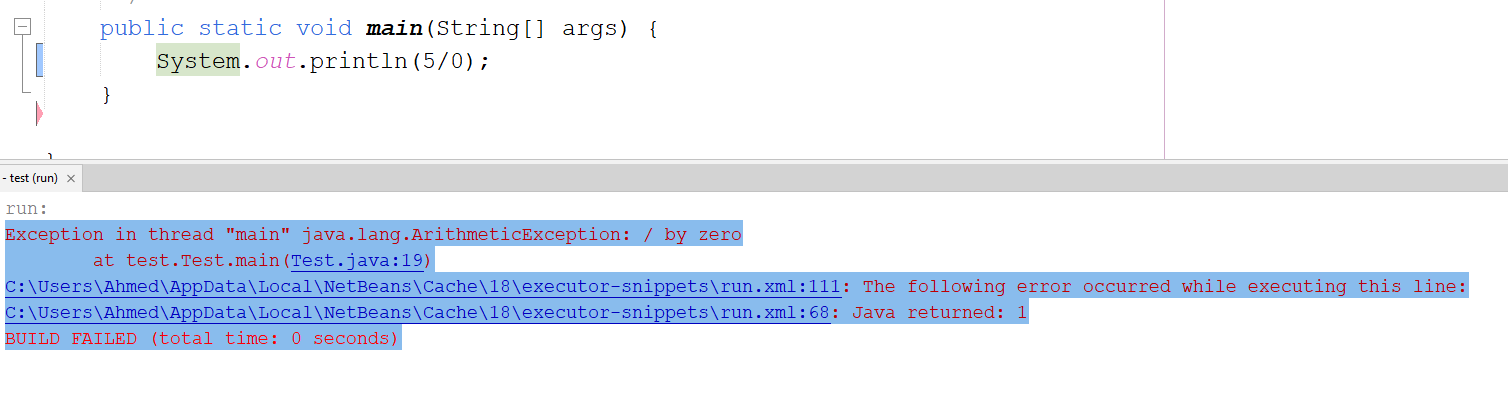
\includegraphics[scale=.4]{exp.png}
\begin{AR}
  كما نري قام بطباعة رسالة حمراء معنها انه حدثت مشكلة اثناء التنفيذ 
  و نحن لا نريد للمتسخدم ان يري رسالة مثل هذه لانه لن يفهم معناها ف علينا ان 
  نقوم بالاخذ في الاعتبار هذه الحالات و هناك مقولة في عالم البرمجة
  تقول 
  \\
  \LR{beware of the lazy and the crazy user}
  مبعني احذر من المستخدم الكسلان و المجنون 
  و المقصود هو المستخدم الذي يدخل قيم غير مقبولة مثلا تطلب منه رقم يدخل لك 
  رموز او نص
  و اكبر مثال نري فيه تعامل جيد مع هذه الحالات هو عند القيام بعمل 
  حساب جديد ف يطلب منك تكتب ال\LR{password} ف يطلب منك خواص محددة لابد من تنفيذها و لايقبل الا عند اتمام جميع الخواص 
\end{AR}
\subsection{try-catch}
\begin{AR}
  الجملة التي سوف نستعملها للتعامل مع ال\LR{Exception} هي ال \LR{try-catch} تكتب هكذا
\end{AR}
\begin{minted}[escapeinside=||]{java}
            try {
              ..........;
            } catch (typeofException ex) {
              ..........;
            }
\end{minted}
\begin{AR}
  نضع داخل ال\LR{try} الاوامر التي نشك انها سوف يحدث فيها مشكلة 
  و نضع داخل ال \LR{catch} الاوامر التي يتم تنفيذها عند حدوث هذه المشكلة
  و داخل اقواس ال\LR{catch} نضع نوع ال\LR{Exception} المتوقع
  \\
  مثال نوع الخطأ الذي يحدث عند القسمة علي صفر هو \LR{ArithmeticException} ف اذا اردنا معالجة مشكلة القسمة علي صفر نكتب الاتي
\end{AR}
\begin{minted}[escapeinside=||]{java}
        try {
            System.out.println(5/0);
        } catch (ArithmeticException ex) {
            System.out.println("you tried to divide by zero");
        }
        
        Output:
              you tried to divide by zero
\end{minted}
\begin{AR}
  نلاحظ انه لم يقم بطباعة اي \LR{Exception} بل قام بطباعة الرسالة التي جهزناها في حالة حدوث هذا الخطأ
  \\
  في حالة انه لو لم يكن هناك اي مشاكل ف سوف يتم تنفيذ بما بداخل ال \LR{try} و لن ينفذ ما بداخل ال \LR{catch}
\end{AR}
\subsection{try-catch-finally}
\begin{AR}
  هناك اضافة يمكن كتابتها مع جملة ال\LR{try-catch} و هي 
  \LR{finally} و يوضع داخلها اوامر يتم تنفيذها في كل الحالات سواء حدث خطأ ام لم يحدث
\end{AR}
\begin{minted}[escapeinside=||]{java}
  try {
      System.out.println(5/0);
  } catch (ArithmeticException ex) {
      System.out.println("you tried to divide by zero");
  }finally{
            System.out.println("hello from Finally");
  }
  
  Output:
        you tried to divide by zero
        hello from Finally
\end{minted}


\section{tips and tricks}
\subsection{constants}
\begin{AR}
  هناك نوع من المتغيرات يسمي الثوابت و كما هو اسمها هي قيمة لا تتغير و تكتب هكذا
\end{AR}
\begin{minted}[escapeinside=||]{java}
    final double pi = 3.14;
\end{minted}
\begin{AR}
  بافاضة كلمة \LR{final} اصبح هذا المتغير ثابت و لايمكن تعديل قيمته في المستقبل
\end{AR}
\subsection{comment}
\begin{AR}
  عند كتابة برنامج كبير علينا وضع بعض الملاحظات علي الاوامر التي نكتبها لكي نتذكر ما الذي تقوم به هذه الاوامر
  \\
  لكتابة اي نص لانريد من البرنامج تنفيذه نقوم بكتابته هكذا
\end{AR}
\begin{minted}[escapeinside=||]{java}
  // line comment
  OR
  /*
  multiple 
  line 
  comment
  */
\end{minted}
\newpage
\subsection{Block}
\begin{AR}
  الاقواس التي تستخدم مع الجمل لكتابة الاكواد داخلها \LR{{ }} تسمي \LR{Block} فعندما نقول \LR{if-block} 
  يقصد بها الاقواس الخاصة بال\LR{if} التي يكتب داخلها الاكواد
  \\
  هناك اختصار اذا كانت الاوامر المكتوبة داخل ال\LR{Block} هي سطر واحد فقط فيمكننا عدم كتابة اقواس ال \LR{Block}
\end{AR}
\begin{minted}[escapeinside=||]{java}
        if (5>3)
          System.out.println("true");
\end{minted}
\begin{minted}[escapeinside=||]{java}
        for (int i = 0; i < 10; i++) 
          System.out.println(i);
\end{minted}
\subsection{Scope}
\begin{AR}
  عند تعريف متغير داخل \LR{Block} ف انه لا يمكن الوصول اليه خارج هذه ال\LR{Block} مثلا في جملة ال \LR{for}
\end{AR}
\begin{minted}[escapeinside=||]{java}
  for (int i = 0; i < 10; i++){ 
    System.out.println(i);
  }
\end{minted}
\begin{AR}
  لا يمكن استدعاء المتغير \LR{i} خارج ال \LR{Block} الخاص بال \LR{for}
\end{AR}
\subsection{code complelation}
\begin{AR}
  يمكنك جعل ال\LR{IDE} الذي تستخدمه يقوم باكمال الاوامر لك عن طريق الضغط علي 
  \LR{ctrl+space}
\end{AR}
\subsection{multiple Variable}
\begin{AR}
  يمكنك تعريف عدد من المتغيرات علي نفس السطر بهذه الطريقة
\end{AR}
\begin{minted}[escapeinside=||]{java}
    int x = 10 , y = 20 , z = 30;
\end{minted}
\subsection{Escape sequences}
\begin{AR}
  يوجد بعض الاختصارات التي يمكن كتابتها في امر الطباعة للقيام بتعديل في التنسيق
\end{AR}
\begin{minted}[escapeinside=||]{java}
  // (1) \t : Inserts a tab space = "    "
  System.out.println("Ahmed\tmohamed");

  output:
        Ahmed    mohamed
\end{minted}
\begin{minted}[escapeinside=||]{java}
  // (2) \n : Inserts a new line
  System.out.println("Ahmed \n mohamed");

  output:
        Ahmed    
        mohamed
\end{minted}
\begin{minted}[escapeinside=||]{java}
  // (3) \" : Inserts a double quote
  System.out.println("\"Ahmed mohamed\"");

  output:
        "Ahmed mohamed"
        
\end{minted}
\begin{minted}[escapeinside=||]{java}
  // (4) \\ : Inserts a backslash
  System.out.println("\\Ahmed mohamed\\");

  output:
        |$\backslash$|Ahmed mohamed|$\backslash$|
        
\end{minted}
\newpage
\section{Arrays}
\begin{AR}
  لنتخيل مجموعة من الصناديق 
\end{AR}
\begin{center}
  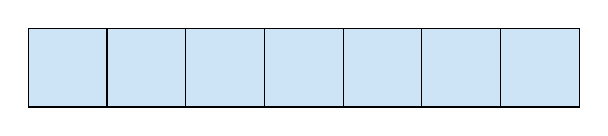
\begin{tikzpicture}
    \draw[fill=theme!20] (-3,0) rectangle (-2,1);
    \draw[fill=theme!20] (-2,0) rectangle (-1,1);
    \draw[fill=theme!20] (-1,0) rectangle (0,1);
    \draw[fill=theme!20] (0,0) rectangle (1,1);    
    \draw[fill=theme!20] (1,0) rectangle (2,1);
    \draw[fill=theme!20] (2,0) rectangle (3,1);
    \draw[fill=theme!20] (3,0) rectangle (4,1);
  \end{tikzpicture}
\end{center}
\begin{AR}
  قمنا بترقيمها بداية من \LR{0} 
\end{AR}
\begin{center}
  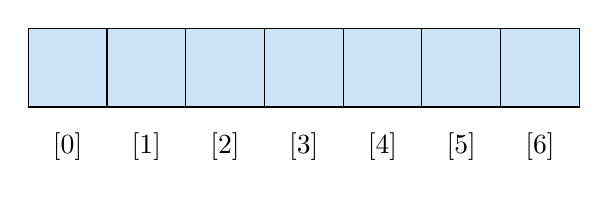
\begin{tikzpicture}
    \draw[fill=theme!20] (-3,0) rectangle (-2,1);
    \draw[fill=theme!20] (-2,0) rectangle (-1,1);
    \draw[fill=theme!20] (-1,0) rectangle (0,1);
    \draw[fill=theme!20] (0,0) rectangle (1,1);    
    \draw[fill=theme!20] (1,0) rectangle (2,1);
    \draw[fill=theme!20] (2,0) rectangle (3,1);
    \draw[fill=theme!20] (3,0) rectangle (4,1);
    \node at (-2.5,-.5) {[0]};
    \node at (-1.5,-.5) {[1]};
    \node at (-.5,-.5) {[2]};
    \node at (.5,-.5) {[3]};
    \node at (1.5,-.5) {[4]};
    \node at (2.5,-.5) {[5]};
    \node at (3.5,-.5) {[6]};
  \end{tikzpicture}
\end{center}
\begin{AR}
  و قمنا بوضع داخل كل صندوق قيمة ما  
\end{AR}
\begin{center}
  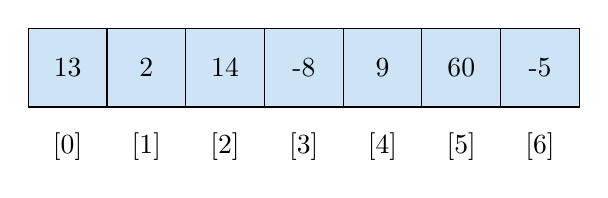
\begin{tikzpicture}
    \draw[fill=theme!20] (-3,0) rectangle (-2,1);
    \draw[fill=theme!20] (-2,0) rectangle (-1,1);
    \draw[fill=theme!20] (-1,0) rectangle (0,1);
    \draw[fill=theme!20] (0,0) rectangle (1,1);    
    \draw[fill=theme!20] (1,0) rectangle (2,1);
    \draw[fill=theme!20] (2,0) rectangle (3,1);
    \draw[fill=theme!20] (3,0) rectangle (4,1);
    \node at (-2.5,-.5) {[0]};
    \node at (-1.5,-.5) {[1]};
    \node at (-.5,-.5) {[2]};
    \node at (.5,-.5) {[3]};
    \node at (1.5,-.5) {[4]};
    \node at (2.5,-.5) {[5]};
    \node at (3.5,-.5) {[6]};

    \node at (-2.5,.5) {13};
    \node at (-1.5,.5) {2};
    \node at (-.5,.5) {14};
    \node at (.5,.5) {-8};
    \node at (1.5,.5) {9};
    \node at (2.5,.5) {60};
    \node at (3.5,.5) {-5};
  \end{tikzpicture}
\end{center}
\begin{AR}
  الان اذا طلبت منك احضار القيمة الموجودة في الصندوق رقم \LR{2}
  سوف تقول انها \LR{14} و بالمثل اذا طلبت اي صندوق اخر 
  \\
  في البرمجة يوجد ما يسمي بال\LR{array} او المصفوفة و هي تماما مثل الذي قمنا بعمله منذ قليل 
  يمكن تخزين مجموعة من القيم او المتغيرات في \LR{array} علي شرط ان يكونوا من نفس النوع فلا يمكن
  تخزين \LR{String} في مصفوفة قمت بتعريفها لكي تحمل قيم \LR{int}
  \\
  الان لنري كيف تكتب ال\LR{array} في الجافا 
\end{AR}
\begin{minted}[escapeinside=||]{java}
      int[] arr = new int[7];
\end{minted}
\begin{AR}
  في هذا الكود قمت بتعريف \LR{array} حجمها \LR{7} بمعني انه يوجد سبع اماكن للتخزين فيها
  \\
  لكي نخزن فيها نكتب الاتي 
\end{AR}
\begin{minted}[escapeinside=||]{java}
      arr[0] = 5;
      arr[3] = 2;
\end{minted}
\begin{AR}
    اقوم بالنداء علي اسم ال\LR{array} ثم اقوم بتحديد المكان الذي اريد التخزين فيه ثم اعطيه القيمة
    \\
    اذا اردنا طباعة عنصر من هذه المصفوفة اقوم فقط بالنداء علي اسمها و اكتب اسم المكان المطلوب 
\end{AR}
\begin{minted}[escapeinside=||]{java}
      System.out.println(arr[3]);

      output:
            2
\end{minted}
\begin{AR}
  و يمكن طباعة جميع عناصر المصفوفة بالستخدام جمل التكرار 
\end{AR}
\begin{minted}[escapeinside=||]{java}
      int[] arr = new int[7];
      arr[0] = 5;
      arr[3] = 2;
      System.out.print("[");
      for (int i = 0; i < 7; i++) {
          System.out.print(arr[i]+",");
      }
      System.out.print("]");

      output:
            [5,0,0,2,0,0,0,]
\end{minted}
\begin{AR}
  لاحظ ان الامكان التي قمنا باعطاء قيم لها لها قيمة بينما القيم التي لم 
  نعطيها قيمة تم تخزين فيها القيمة الافتراضية للمتغير \LR{int} و هي ال \LR{0}
  \\
  اذا قمنا بتكرار الكود وجعلنا ال\LR{array} نوعها \LR{String}
\end{AR}
\begin{minted}[escapeinside=||]{java}
      String[] arr = new String[7];
      arr[0] = "Ahmed";
      arr[3] = "Mohamed";
      System.out.print("[");
      for (int i = 0; i < 7; i++) {
          System.out.print(arr[i]+",");
      }
      System.out.print("]");

      output:
            [Ahmed,null,null,Mohamed,null,null,null,]
\end{minted}
\begin{AR}
  و ذلك بسبب ان القيمة الافتراضية لل\LR{String} هي \LR{null}
  \\
  يمكن التعديل علي الاكواد السابقة و جعل الشرط الموجود في ال\LR{for} يكتب هكذا
\end{AR}
\begin{minted}[escapeinside=||]{java}
  String[] arr = new String[7];
  arr[0] = "Ahmed";
  arr[3] = "Mohamed";
  System.out.print("[");
  for (int i = 0; i < arr.length; i++) {
      System.out.print(arr[i]+",");
  }
  System.out.print("]");

  output:
        [Ahmed,null,null,Mohamed,null,null,null,]
\end{minted}
\begin{AR}
  قمت استخدمت \LR{arr.length} بدل من \LR{7} لان \LR{arr.length} تساوي حجم المصفوفة
  \\
  لكن لماذا علينا ان لا نخرج خارج حدود المصفوفة لماذا لا يمكن كتابة 
\end{AR}
\begin{minted}[escapeinside=||]{java}
  String[] arr = new String[7];
  arr[-1] = "Ahmed";
  OR
  arr[50] = "Mohamed";
\end{minted}
\begin{AR}
  اذا قمت بالنداء علي مكان خارج حدود المصفوفة و التي في مثالنا هذا \LR{0-6} فان البرنامج يقوم بعمل \LR{Exception} من النوع \LR{ArrayIndexOutOfBoundsException} و معناها اننا خرجنا خارج حدود المصفوفة
  و هذا لان ال\LR{array} حجمها يكون ثابت بمجرد كتابة قيمته عند التعريف لا يمكن تغييرها
  \\
  يوجد طريقة اخري لتعريف ال\LR{array} و هي بالستخدام اقواس المجموعة هكذا
\end{AR}
\begin{minted}[escapeinside=||]{java}
        String[] arr = {"ahmed", "Mohamed"};
        System.out.print("[");
        for (int i = 0; i < arr.length; i++) {
            System.out.print(arr[i] + ",");
        }
        System.out.print("]");
    output:
          [ahmed,Mohamed,]
\end{minted}
\begin{AR}
  في هذه الطريقة حجم ال\LR{array} يتم تحديده حسب عدد القيم المكتوبة داخل اقواس المجموعة
\end{AR}


\begin{example}
  \RL{
  قم بعمل برنامج يطلب من المستخدم اسماء ثلاث طلاب و درجاتهم ثم يقوم بطباعتهم 
  }
              
  \begin{center}
    ------ \textcolor{Solution}{Solution} ------ 
  \end{center}
  \begin{minted}[escapeinside=||]{java}
  Scanner s = new Scanner(System.in);
  String[] names = new String[3];
  double[] grades = new double[3];
  for (int i = 0; i < names.length; i++) {
      System.out.println("Enter Student number " + (i+1) +" name:");
      names[i]=s.next();
      System.out.println("Enter Student number " + (i+1) +" grade:");
      grades[i]=s.nextDouble();
  }
  for (int i = 0; i < names.length; i++) {
      System.out.println("Student number "+ (i+1) +" name: "+names[i] + " ,grade: " +grades[i] );
  }

  output:
        Enter Student number 1 name:
        |\textcolor{red}{adam}|
        Enter Student number 1 grade:
        |\textcolor{red}{100}|
        Enter Student number 2 name:
        |\textcolor{red}{mohamed}|
        Enter Student number 2 grade:
        |\textcolor{red}{95.8}|
        Enter Student number 3 name:
        |\textcolor{red}{ahmed}|
        Enter Student number 3 grade:
        |\textcolor{red}{80.99}|
        Student number 1 name: adam ,grade: 100.0
        Student number 2 name: mohamed ,grade: 95.8
        Student number 3 name: ahmed ,grade: 80.99
  \end{minted}
\end{example}
\begin{minipage}[h]{1\textwidth}
\begin{example}
  \RL{
  قم بعمل برنامج يقوم بحساب مجموع عناصر مصفوفة
  }
              
  \begin{center}
    ------ \textcolor{Solution}{Solution} ------ 
  \end{center}
  \begin{minted}[escapeinside=||]{java}
        double[] nums = {6.5,87,51.41,64.3,15.4};
        double sum = 0;
        for (int i = 0; i < nums.length; i++) {
            sum+= nums[i];
        }
        System.out.println(sum);

        output:
              224.6
  \end{minted}
\end{example}
\end{minipage}
\begin{task}
  \begin{AR}
    قم بعمل برنامج يقوم بحساب متوسط عناصر مصفوفة
  \end{AR}
\end{task}
\begin{example}
  \RL{
  قم بعمل برنامج يقوم بالبحث عن قيمة ما داخل مصفوفة
  }
              
  \begin{center}
    ------ \textcolor{Solution}{Solution} ------ 
  \end{center}
  \begin{minted}[escapeinside=||]{java}
        int[] A = {6,99,9,26,62,3,18,91,33,22,17,63,35,34,98,52,1,86,71,58};
        int searchvalue = 17;
        int position = -1;
        for(int i = 0; i < A.length; i++) {
            if (A[i] == searchvalue) {
                position = i;
                break;
            }
        }
        if (position != -1) {
            System.out.println("found in position " + position);
        } else {
            System.out.println("not found");
        }

        output:
              found in position 10  
  \end{minted}
\end{example}
\begin{task}
  \begin{AR}
    قم بعمل برنامج بقوم بمقارنة عناصر مصفوفتان و يكتب اذا كانوا متساويين او لا 
  \end{AR}
\end{task}
\subsection{Arrays class}
\begin{AR}
يوجد في الجافا \LR{class} يوجد به العديد من الادوات المفيدة التي يمكن ان تسهل عليها العمل بالمصفوفات
\\
يتم استدعاء بكتابة
\end{AR}
\begin{minted}[escapeinside=||]{java}
  import java.util.Arrays;
\end{minted}

\begin{AR}
مثل تماما استدعاء ال \LR{Scanner} و كما سوف نري هذه بعض الاوامر الموجودة في هذا ال\LR{class}
\end{AR}
\begin{minted}[escapeinside=||]{java}
  Arrays.equals(A, B);
\end{minted}
\begin{AR}
  يستخدم هذا الامر لفحص اذا كانت \LR{A} و \LR{B} متساويتان ام لا ويقوم بارجاع قيمة \LR{true} او \LR{false} حسب ناتج المقارنة
\end{AR}
\begin{minted}[escapeinside=||]{java}
  Arrays.fill(A, value);
\end{minted}
\begin{AR}
  بقوم بملئ جميع خانات المصفوفة \LR{A} بالقيمة \LR{value}
\end{AR}
\begin{minted}[escapeinside=||]{java}
  Arrays.sort(A);
\end{minted}
\begin{AR}
  بقوم بترتيب المصفوفة \LR{A} ترتيب تصاعدي
\end{AR}
\begin{minted}[escapeinside=||]{java}
  Arrays.toString();
\end{minted}
\begin{AR}
  بقوم بارجاع \LR{String} يحتوي علي عناصر المصفوفة \LR{A} مكتوبة بشكل مرتب
\end{AR}

\begin{example}
  \RL{
  قم بعمل برنامج يقوم بترتيب مصفوفة
  }
              
  \begin{center}
    ------ \textcolor{Solution}{Solution} ------ 
  \end{center}
  \begin{minted}[escapeinside=||]{java}
        int[] A = {6,99,9,26,62,3,18,91,33,22,17,63,35,34,98,52,1,86,71,58};
        Arrays.sort(A);
        System.out.println(Arrays.toString(A));

        output:
              [1, 3, 6, 9, 17, 18, 22, 26, 33, 34, 35, 52, 58, 62, 63, 71, 86, 91, 98, 99]
  \end{minted}
\end{example}
\begin{example}
  \RL{
  قم بعمل برنامج يقوم بدمج مصفوفاتان داخل مصفوفة واحدة 
  }       
  \begin{center}
    ------ \textcolor{Solution}{Solution} ------ 
  \end{center}
  \begin{minted}[escapeinside=||]{java}
        int[] A = {1,2,3,4,5};
        int[] B = {6,7,8,9,10};
        int[] merge = new int[A.length+B.length];

        for(int i = 0; i < A.length; i++) {
            merge[i] = A[i];
        }
        for(int i = 0; i < B.length; i++) {
            merge[i+A.length] = B[i];
        }
        System.out.println(Arrays.toString(merge));

        output:
              [1, 2, 3, 4, 5, 6, 7, 8, 9, 10]
  \end{minted}
\end{example}




%%%%%%%%%%%%%%%%%%%%%%    Done till here    %%%%%%%%%%%%%%%%%%%%
\subsection{Char Array}
%sysout(array name) = tostring
%ASCII code
\begin{AR}
يوجد نوع خاص من المصفوفات و هي مصفوفة الاحرف و التي يتم تخزين فيها قيم 
\LR{char} فقط
المميز في هذه المصفوفة انه اذا قمت بطباعتها تقوم بطباعة الاحرف بجانب بعضها في كلمة واحدة
\end{AR}
\begin{minted}[escapeinside=||]{java}
  char arr[] = {'a','$','c'};
  System.out.println(arr);

  output:
        a$c
\end{minted}
\begin{AR}
    و ايضا يمكن وضع بداخلها\LR{ASCII Codes} و سوف تتعرف عليها
\end{AR}
\begin{minted}[escapeinside=||]{java}
  char arr[] = {97,37,99};
  System.out.println(arr);

  output:
        a%c
\end{minted}

\begin{figure*}[b]
  %\begin{minipage}[h]{1\textwidth}
  \begin{enrichment*}{ASCII Codes}
  \begin{AR}
    اكواد الاسكي او ال \LR{ASCII Codes} هي مجموعة من الارقم يمرز كل رقم منها الي حرف ما او رمز ما 
    تم وضعها لكي نستطيع كتابة الرموز الغير موجودة علي الكيبورد مثل \LR{$\Sigma , \gamma , \spadesuit , \clubsuit , \measuredangle $} بالاضافة الي 
    توحيد طريقة كتابة هذه الرموز
  \end{AR}
\end{enrichment*}
%\end{minipage}
\end{figure*}
\subsection{Enhanced for}
\begin{AR}
    الان بعد ان تعرفنا علي المصفوفات سوف نتعرف علي طريقة اسهل لكي نمر علي 
    كل عناصر المصفوفة و هي ال \LR{for-Each} و التي اذا ترجمناها معناها سوف يكون \LR{"}لكل\LR{"} اي
    لكل عنصر في المصفوفة و الان لنري كيف تكتب
\end{AR}
\begin{minted}[escapeinside=||]{java}
      int arr[] = {97,37,99};
      for (int element : arr) {
          System.out.println(element);
      }
      output:
            97
            37
            99
\end{minted}  
\begin{AR}
    في الكود السابق قمت بعمل مصفوفة ارقام و طبعتها لكن 
    باستخدام ال \LR{for-Each} و هي مثل ال \LR{for} العادية لكن بدون عداد و تتوقف عندما تنتهي 
    عناصر المصفوفة الموجودة في اقواسها
\end{AR}
\subsection{Multi-Dimensional Array}
\begin{AR}
    الان بعد ان عرفنا المصفوفة التي مكونة من بعد واحد و تم تمثيله علي شكل صف 
\end{AR}
\begin{center}
  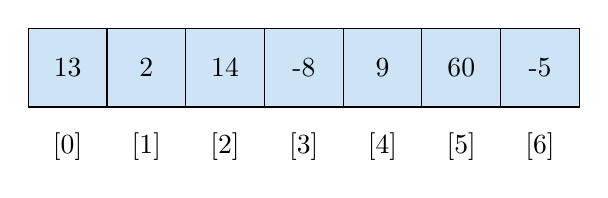
\begin{tikzpicture}
    \draw[fill=theme!20] (-3,0) rectangle (-2,1);
    \draw[fill=theme!20] (-2,0) rectangle (-1,1);
    \draw[fill=theme!20] (-1,0) rectangle (0,1);
    \draw[fill=theme!20] (0,0) rectangle (1,1);    
    \draw[fill=theme!20] (1,0) rectangle (2,1);
    \draw[fill=theme!20] (2,0) rectangle (3,1);
    \draw[fill=theme!20] (3,0) rectangle (4,1);
    \node at (-2.5,-.5) {[0]};
    \node at (-1.5,-.5) {[1]};
    \node at (-.5,-.5) {[2]};
    \node at (.5,-.5) {[3]};
    \node at (1.5,-.5) {[4]};
    \node at (2.5,-.5) {[5]};
    \node at (3.5,-.5) {[6]};

    \node at (-2.5,.5) {13};
    \node at (-1.5,.5) {2};
    \node at (-.5,.5) {14};
    \node at (.5,.5) {-8};
    \node at (1.5,.5) {9};
    \node at (2.5,.5) {60};
    \node at (3.5,.5) {-5};
  \end{tikzpicture}
\end{center}
\begin{AR}
  يمكننا عمل مصفوفة مكونة من بعدين و يكون شكلها هكذا
\end{AR}
\begin{center}
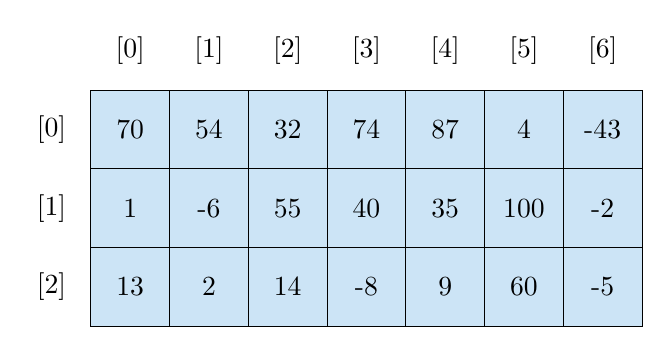
\begin{tikzpicture}
  \draw[fill=theme!20] (-3,2) rectangle (-2,3);
  \draw[fill=theme!20] (-2,2) rectangle (-1,3);
  \draw[fill=theme!20] (-1,2) rectangle (0,3);
  \draw[fill=theme!20] (0,2) rectangle (1,3);    
  \draw[fill=theme!20] (1,2) rectangle (2,3);
  \draw[fill=theme!20] (2,2) rectangle (3,3);
  \draw[fill=theme!20] (3,2) rectangle (4,3);

  \draw[fill=theme!20] (-3,1) rectangle (-2,2);
  \draw[fill=theme!20] (-2,1) rectangle (-1,2);
  \draw[fill=theme!20] (-1,1) rectangle (0,2);
  \draw[fill=theme!20] (0,1) rectangle (1,2);    
  \draw[fill=theme!20] (1,1) rectangle (2,2);
  \draw[fill=theme!20] (2,1) rectangle (3,2);
  \draw[fill=theme!20] (3,1) rectangle (4,2);

  \draw[fill=theme!20] (-3,0) rectangle (-2,1);
  \draw[fill=theme!20] (-2,0) rectangle (-1,1);
  \draw[fill=theme!20] (-1,0) rectangle (0,1);
  \draw[fill=theme!20] (0,0) rectangle (1,1);    
  \draw[fill=theme!20] (1,0) rectangle (2,1);
  \draw[fill=theme!20] (2,0) rectangle (3,1);
  \draw[fill=theme!20] (3,0) rectangle (4,1);
  \node at (-2.5,3.5) {[0]};
  \node at (-1.5,3.5) {[1]};
  \node at (-.5,3.5) {[2]};
  \node at (.5,3.5) {[3]};
  \node at (1.5,3.5) {[4]};
  \node at (2.5,3.5) {[5]};
  \node at (3.5,3.5) {[6]};

  \node at (-3.5,2.5) {[0]};
  \node at (-3.5,1.5) {[1]};
  \node at (-3.5,.5) {[2]};

  \node at (-2.5,.5) {13};
  \node at (-1.5,.5) {2};
  \node at (-.5,.5) {14};
  \node at (.5,.5) {-8};
  \node at (1.5,.5) {9};
  \node at (2.5,.5) {60};
  \node at (3.5,.5) {-5};

  \node at (-2.5,1.5) {1};
  \node at (-1.5,1.5) {-6};
  \node at (-.5,1.5) {55};
  \node at (.5,1.5) {40};
  \node at (1.5,1.5) {35};
  \node at (2.5,1.5) {100};
  \node at (3.5,1.5) {-2};

  \node at (-2.5,2.5) {70};
  \node at (-1.5,2.5) {54};
  \node at (-.5,2.5) {32};
  \node at (.5,2.5) {74};
  \node at (1.5,2.5) {87};
  \node at (2.5,2.5) {4};
  \node at (3.5,2.5) {-43};
\end{tikzpicture}
\end{center}
\begin{AR}
    علاوة علي ذلك يمكننا عمل مصفومة من مكونة من اي عدد من الابعاد
    لكي نقوم بتعريف مصفوفة من البعد الثاني نكتب الاتي 
\end{AR}
\begin{minted}[escapeinside=||]{java}
  int arr[][] = {
        {70, 54, 32, 74, 87, 4, -43},
        {1, -6, 55, 40, 35, 100, -2},
        {13, 2, 14, -8, 9, 60, -5}
        };
\end{minted}
\begin{AR}
  لكي نمر علي كل عنصر في هذه المصفوفة سوف نحتاج \LR{nested loop} 
\end{AR}

\begin{minted}[escapeinside=||]{java}
  int arr[][] = {
        {70, 54, 32, 74, 87, 4, -43},
        {1, -6, 55, 40, 35, 100, -2},
        {13, 2, 14, -8, 9, 60, -5}
        };
        for (int[] is : arr) {
            for (int i : is) {
                System.out.print(i+" ");
            }
            System.out.println();
        }

      output:
            70 54 32 74 87 4 -43 
            1 -6 55 40 35 100 -2 
            13 2 14 -8 9 60 -5 
\end{minted}

\begin{AR}
  و اذا اردت عنصر ما بالتحدد اقوم بالنداء عليه عن طريق مكانه اقوم اولا بتحديد رقم الصف الموجود فيه ثم رقم العمود
\end{AR}

\begin{minted}[escapeinside=||]{java}
  int arr[][] = {
        {70, 54, 32, 74, 87, 4, -43},
        {1, -6, 55, 40, 35, 100, -2},
        {13, 2, 14, -8, 9, 60, -5}
        };
  System.out.println(arr[1][2]);

      output:
            55
\end{minted}

\section{Methods}
\begin{AR}
في هذا الجزء سوف نتحدث عن مفهوم جديد و هو ال \LR{methods}
\end{AR}
\subsection{What is Method}
\begin{AR}
\LR{method} او \LR{function} او دالة جميعها مسميات لنفس الشئ
و هي  بديل للذي كنا نفعله في السابق حيث كنا نكتب الاوامر كلها في مكان واحد و كلها 
مع بعضها و يصعب التفريق بينهم و معرفة مهمة كل جزء 
الان يمكننا وضع الاوامر الخاصة بنا في دوال مختلفة و النداء عليها وقت ما نشاء بقدر ما نشاء
\\\\
لكي تنشاء \LR{method} تكتب الاتي 
\end{AR}
\begin{minted}[escapeinside=||]{java}
  public static void mymethod(){
    
  }
\end{minted}
\begin{AR}
اترك \LR{public} و \LR{static} و \LR{void} سوف نتعمق في معناهم في وقت لاحق كل ما عليك معرفته هو
ان \LR{method} تكتب هكذا و \LR{mymethod} هو اسمها
\\
الان لنرا كيف تعمل مثلا لنقوم بعمل دالة تقوم بطباعة \LR{"hi"}
\end{AR}
\begin{minted}[escapeinside=||]{java}
  public static void sayhi(){
        System.out.println("hi");
    }
    public static void main(String[] args) {
        sayhi();
    }

    output:
            hi
\end{minted}
\begin{AR}
الان اذا اردنا تكرار تنفيذ الامر ليس علينا الا ان ننادي علي اسم الدالة مجددا
\end{AR}
\begin{minted}[escapeinside=||]{java}
  public static void sayhi(){
        System.out.println("hi");
    }
    public static void main(String[] args) {
        sayhi();
        sayhi();
        sayhi();
    }

    output:
            hi
            hi
            hi
\end{minted}
\subsection{Method With Parameters}
\begin{AR}
بعد ان تعرفنا علي ال \LR{method} و كيفية عملها الان سوف نري تعديل بسيط علي شكلها 
و هو اننا سوف نضيف مكان في الدالة لادخال متغير
\end{AR}
\begin{minted}[escapeinside=||]{java}
  public static void mymethod(type var1 , type var2 ,...){
    
  }
\end{minted}
\begin{AR}
و علي هذا الشكل يمكننا اضافة اي عدد من المتغيرات للدالة بمجرد ان نكتب نوع المتغير 
و اسمه في هذه الاقواس يمكننا استدعائه داخل الدالة و تنفيذ عليه الاوامر لنري بعض الامثلة 
\\
دالة تقوم بجمع رقمين و تطبعهم 
\end{AR}
\begin{minted}[escapeinside=||]{java}
  public static void add(int x , int y){
        System.out.println(x+y);
    }
    public static void main(String[] args) {
        add(5,6);
        add(1,-2);
        add(23,0);
    }

    output:
            11
            -1
            23
\end{minted}
\begin{AR}
  دالة تقوم باخذ نصف قطر دائرة و تقوم بحساب محيطها
\end{AR}
\begin{minted}[escapeinside=||]{java}
    public static void circle_perimeter(double radius){
        System.out.println(2*3.14*radius);
    }
    public static void main(String[] args) {
        circle_perimeter(5);
    }

    output:
          31.4
\end{minted}
\begin{AR}
  دالة تقوم باخذ نصف قطر دائرة و تقوم بحساب مساحتها
\end{AR}
\begin{minted}[escapeinside=||]{java}
  public static void circle_area(double radius){
      System.out.println(3.14*radius*radius);
  }
  public static void main(String[] args) {
    circle_area(5);
  }

  output:
        78.5
\end{minted}
\newpage
\subsection{void vs return method}
\begin{AR}
  يمكننا الان التحدث عن 
  النوعين الاساسيين لاي \LR{method} و هم \LR{return method} و \LR{void method}
  جميع الدوال التي قمنا بعملها الي الان هي دوال من النوع \LR{void} و هي دوال تقوم بعمل مهمة او تنفيذ اوامر 
  فقط و ينتهي دورها لا تقوم بارجاع قيمة بعد انتهائها اما \LR{return method} تقوم بارجاع قيمة او متغير بشكل عام بعد
  الانتهاء من تنفيذ الاوامر بداخلها لنري مثال علي ذلك\\
  سوف نقوم بعمل الدالة التي تقوم بحساب مساحة الدائرة لكن هذه المرة لن نقوم 
  بطباعة القيمة بل سوف نرجعها 
\end{AR}
\begin{minted}[escapeinside=||]{java}
  public static double circle_area(double radius){
      return 3.14*radius*radius ;
  }
  public static void main(String[] args) {
    double area = circle_area(5);
    System.out.println(area);
  }

  output:
        78.5
\end{minted}
\begin{AR}
الفرق بين الطريقة الاول و الطريقة الثانية اننا في هذه الحالة قمنا بارجاع قمة المساحة 
باستخدام الامر \LR{return} بدلا من طباعتها مباشرة و نستطيع بعدها بتخزين هذه القيمة التي تم ارجاعها في متغير 
او القيام بعمليات اخري عليها كما نشاء و قمنا ايضا بتغيير كلمة \LR{void} الموجودة في تعريف ال \LR{method} لنوع 
المتغير الذي نريد ارجاعه 
\end{AR}

\section{Classes}
\begin{AR}
سوف نتحدث عن موضوع جديد الان و هو ال \LR{classes} ما هي و بعض ال \LR{classes} المهمة في لغة ال \LR{Java}
\end{AR}
\subsection{What is Class}
\begin{AR}
  ترجمة كلمة \LR{class} بطريقة حرفية تعني تصنيف او نوع 
  و هذا المعني يصف بشكل جزئي اهميتها في لغات البرمجة حيث انه يستخدم في انشاء متغيرات من انواع 
  مختلفة عن الانواع الاساسية \LR{(integer , String , double,...)} 
  مثلا يمكننا انشاء \LR{class} اسمه \LR{car} و بعدها نستطيع ان نصنع منه 
  متغيرات من نفس هذا النوع 
  \\\\
  قد تعرضنا سابقا لل \LR{classes} لكن لم نلاحظها مثلا عند تعريف \LR{array} او عند عمل \LR{Scanner} 
  بل من البداية اذا انشأت مشروع جديد سوف تجد انه يضعه داخل \LR{class} 
  \\\\
  هذه سوف تكون مجرد مقدمة عن ال \LR{classes} لانه سوف نتحدث عنها بتعمق اكتر في جزء البرمجة الشيئية \LR{OOP}
\end{AR}
\subsection{usefull Classes}
\begin{AR}
الان سوف نري بعض ال \LR{classes} المفيدة و التي تحتوي الكتير من الادوات الاساسية 
التي تمكننا من اختصار الوقت عند البرمجة 
\end{AR}
\subsubsection{Scanner Class}
\begin{AR}
تعرضنا لهذا ال\LR{class} من قبل عندما كنا نريد قراءة قيمة من المستخدم 
كنا نقوم بتعريف \LR{object} منه
\end{AR}
\begin{minted}[escapeinside=||]{java}
  Scanner s = new Scanner(System.in);
\end{minted}
\begin{AR}
  و اذا اردنا قراءة رقم صحيح 
\end{AR}
\begin{minted}[escapeinside=||]{java}
  int a = s.nextInt();
\end{minted}
\begin{AR}
  و اذا اردنا قراءة كلمة 
\end{AR}
\begin{minted}[escapeinside=||]{java}
  String b = s.next();
\end{minted}
\begin{AR}
  و اذا اردنا قراءة نص
\end{AR}
\begin{minted}[escapeinside=||]{java}
  String c = s.nextLine();
\end{minted}
\begin{AR}
  و اذا اردنا قراءة قيمة كسرية او عشرية 
\end{AR}
\begin{minted}[escapeinside=||]{java}
  double d = s.nextDouble();
\end{minted}
\begin{AR}
  و اذا اردنا قراءة قيمة منطقية
\end{AR}
\begin{minted}[escapeinside=||]{java}
  boolean e = s.nextBoolean();
\end{minted}
\subsubsection{Math Class}
\begin{AR}
هذا ال\LR{class} يحتوي علي معظم العمليات الرياضية فيمكننا من خلاله 
\\
استخدام ثابت اويلر 
\end{AR}
\begin{minted}[escapeinside=||]{java}
Math.E  
\end{minted}
\begin{AR}
  استخدام الثابت \LR{PI} 
\end{AR}
\begin{minted}[escapeinside=||]{java}
Math.PI  
\end{minted}
\begin{AR}
  حساب القيمة المطلقة 
\end{AR}
\begin{minted}[escapeinside=||]{java}
Math.abs(-5)  
\end{minted}
\begin{AR}
  حساب الاكبر بين رقمين
\end{AR}
\begin{minted}[escapeinside=||]{java}
Math.max(5, 2)
\end{minted}
\begin{AR}
  حساب الاصغر بين رقمين
\end{AR}
\begin{minted}[escapeinside=||]{java}
Math.min(5, 2)  
\end{minted}
\begin{AR}
  حساب الاس 
\end{AR}
\begin{minted}[escapeinside=||]{java}
Math.pow(9, 2)  
\end{minted}
\begin{AR}
  حساب الجزر 
\end{AR}
\begin{minted}[escapeinside=||]{java}
Math.sqrt(0)  
\end{minted}
\begin{AR}
  تحويل الزوايا من القياس الستيني للقياس الدائري و العكس 
\end{AR}
\begin{minted}[escapeinside=||]{java}
Math.toDegrees(3.14)
Math.toRadians(180)  
\end{minted}

\subsubsection{Random Class}
\begin{AR}
يمكننا استخدام هذا ال \LR{class} في اختيار رقم عشوائي داخل فترة محددة 
\end{AR}
\begin{minted}[escapeinside=||]{java}
Random r = new Random();
r.nextInt(0, 100)
\end{minted}
\newpage
%%%%%%%%%%%%%%%%%%%%%%%%%%%%%%%%%%%%%%%%%%%%%%%%%%%%%%
%%%%%%%%%%%%%%%%%%%%%%%%%%%%%%%%%%%%%%%%%%%%%%%%%%%%%%
%%%%%%%%%%%%%%%%%%%%%%%%%%%%%%%%%%%%%%%%%%%%%%%%%%%%%%
%%%%%%%%%%%%%%%%%%%%%%%%%%%%%%%%%%%%%%%%%%%%%%%%%%%%%%
\chapterimage{chapters_cover.jpg}
\chapter{Object Oriented Programming (OOP)}
\thispagestyle{empty}
\section{Introduction}
\subsection{what is package}
\subsection{what is Class}
\subsection{what is Object}
\section{Getting Started with OOP}
\subsection{Create Class}
\subsection{Create Object from Class}
\subsection{Class with Atrributes}
\subsection{Class with Methods}
\section{Encapsolation(access modifiers)}
\section{Constractor with/out parameters}
\section{polymorphism}
\section{OverLoad}
\section{Override}
\section{inheritance}
\section{Abstraction}
\section{Interface}
\section{static methods}
\section{Nested class}
\section{Generic class}
\section{Anonymous class}
\section{Enum}
\section{Threads}
%%%%%%%%%%%%%%%%%%%%%%%%%%%%%%%%%%%%%%%%%%%%%%%%
\LR{}
\begin{AR}

\end{AR}
\begin{minted}[escapeinside=||]{java}
  
\end{minted}

\end{document}